\documentclass[twocolumn,twoside,openright]{report}
\usepackage{standalone}
\usepackage[a4paper,verbose, margin=15mm]{geometry}
\usepackage{enumitem,graphicx,tabularray,subcaption}
\usepackage[font={small,sf}]{caption}
\usepackage{fdsymbol}
\usepackage{awesomebox}
\usepackage{titlesec}
\usepackage{lmodern}
\usepackage[T1]{fontenc}
\usepackage{tikz}
\usepackage{tkz-euclide}
\usetikzlibrary{intersections,shapes.arrows,arrows.meta}
\usetikzlibrary{decorations.pathmorphing,circuits.ee.IEC}

\pdfinfo{
	/Title (Unoffical NABU How-To Guide)
	/Author (DT)
	/Subject (NABU Personal Computer How-To Guide)
	/Keywords (Unofficial, NABU Personal Computer, HowTo, How-To, Minor Repairs)
}

\newcommand*{\blankpage}{%
	\onecolumn
	\vspace*{\fill}
	\begin{center}
		This page intentionally left blank.
	\end{center}
	\vspace{\fill}
}
\makeatletter
\renewcommand*{\cleardoublepage}{\clearpage\if@twoside \ifodd\c@page\else
	\blankpage
	\thispagestyle{empty}
	\newpage
	\if@twocolumn\hbox{}\newpage\fi\fi\fi
}
\makeatother
\newcommand\bbox[2][1mm]{
	\tikz[baseline=(X.base)]
	\node (X) [draw, shape=rectangle, rounded corners=#1, inner sep=1] {\strut #2};
}
\newcommand\Ground{%
	\mathbin{\text{\begin{tikzpicture}[circuit ee IEC,yscale=0.6,xscale=0.5]
				\draw (0,2ex) to (0,0) node[ground,rotate=-90,xshift=.65ex] {};
	\end{tikzpicture}}}%
}
\newcommand{\difficulty}[1]{
	{\color{red}\faWrench}
	{\ifnum#1>1{\color{red}\faWrench}\else\color{gray}\faWrench\fi}
	{\ifnum#1>2{\color{red}\faWrench}\else\color{gray}\faWrench\fi}
	{\ifnum#1>3{\color{red}\faWrench}\else\color{gray}\faWrench\fi}
	{\ifnum#1>4{\color{red}\faWrench}\else\color{gray}\faWrench\fi}
}
\newcommand\frontmatter{
	\cleardoublepage
	\pagenumbering{roman}
}
\newcommand\mainmatter{
	\cleardoublepage
	\pagenumbering{arabic}
}

\titleformat{\chapter}{\normalfont\LARGE\bfseries}{\thechapter}{1em}{}
\titlespacing*{\chapter}{0pt}{3.5ex plus 1ex minus .2ex}{2.3ex plus .2ex}
\titleformat{\section}{\normalfont\large\bfseries}{\thesection}{.5em}{}

\setlength{\columnsep}{1cm}
\setlist[enumerate,1]{wide, labelwidth=!, labelindent=0pt, itemsep=0pt}

\begin{document}

\frontmatter

\begin{titlepage}
	\null\vskip4em
	\begin{figure}[h]
		\centering
		
\includegraphics[scale=0.8]{images/NABU-logo.png}
	\end{figure}
	\vskip4em
	\begin{center}
		{\fontfamily{cmr}\fontsize{36pt}{40pt}\selectfont \textbf{Unofficial How-To Guide}}
		\vfill
		%{\huge NABU Users Group}
	\end{center}
\end{titlepage}

\onecolumn\null\vfill
\section*{Disclaimer}
Every effort has been made to ensure the accuracy of the information contained in this document. The information presented within is accurate at the time of publication.  Whilst every effort is made to provide accurate information, no warranty or fitness is provided or implied, and the authors and publishers shall have neither liability nor responsibility to any person or entity with respect to any loss or damages arising from its use.
All trademarks, logos and brand names are the property of their respective owners. All company, product and service names mentioned in this document are for identification purposes only. Use of these names, trademarks and brands does not imply endorsement.

\section*{License}
This work is licensed under the Creative Commons Attribution-NonCommercial 4.0 International License. To view a copy of this license, visit http://creativecommons.org/licenses/by-nc/4.0/ or send a letter to Creative Commons, PO Box 1866, Mountain View, CA 94042, USA.
\begin{figure}[h!]
	
\includegraphics[width=3cm]{images/by-nc.png}
\end{figure}

\vskip2em
\noindent ~This version April 2023\par\vskip.33em
\noindent\bbox[0mm]{10 9 8 7 6 5 4 3\hskip1em27 26 25 24 23}

\clearpage
\tableofcontents
\listoffigures
\chapter*{Introduction}
\addcontentsline{toc}{chapter}{Introduction}

This `Unofficial How-To Guide' provides step-by-step instructions for a range of tasks, including making cables, unjamming fans, replacing power supplies, and so on. It draws on the personal experience of the authors and the combined skills and knowledge of users of the NABU forum.\footnotemark  The tasks described range from simple \mbox{(\difficulty{1})}, requiring few skills or tools, to fiendish \mbox{(\difficulty{5})}, requiring considerable experience or specialist tools.

\vskip.25em
This guide is `unofficial` because by the time of its creation, the NABU Manufacturing Corp. had been out of business for almost 40 years and so was in no position to sanction its publication. It is also `unofficial' because no one person, or even a group of people, can claim to speak for the NABU community. In many respects, this guide is a joint effort, based on the contributions from numerous people. And while the instructions in this guide are believed to be correct, they are in no way official or even the only way to achieve the stated objectives. Which leads into the final reason for this guide being `unofficial'. If through following any of the instructions in this guide you damage your NABU system or anything else, or hurt yourself or others, you will have no one to blame but yourself. Like many things in life, this guide comes with no guarantees, implied or otherwise. That said -- and while there are \textit{definitely absolutely no guarantees!} -- if you \textit{do} run into problems, you \textit{may} find solace and potentially even solutions in the NABU forum.

\vskip.25em
Finally, if you would like to provide feedback on this guide, either because you've spotted an error of some kind, or because you have one or more suggestions, or for any other reason, please raise a Github `issue' at \mbox{<https://github.com/dimitrit/nabu-howto/issues>}.
\footnotetext{The NABU forum is hosted by the RetroNet team at <https://forums.nabu.ca>.}

\vskip2.5em
\null\hspace{.66\linewidth} DT, April 2023



\mainmatter
\twocolumn[\begin{@twocolumnfalse}
	\chapter{Freeing a stuck fan\hfill\difficulty{2}}
	In many `New Old Stock' (NOS) NABU Personal Computers the fan either doesn't spin freely or is completely stuck. Several fixes have been suggested, including bending fan blades or filing down the fan tips. Following is a simpler and less destructive solution. Alternatively, the fan can be replaced following the instructions in Section \ref{sec:fan-replacement}, `Replacing the NABU fan assembly' on page \pageref{sec:fan-replacement}.
	\vskip1em
\end{@twocolumnfalse}]
\section{Removing the fan}
\awesomebox[red]{2pt}{\faBolt}{red}{To prevent electric shock, you \textbf{must} disconnect your NABU Personal Computer from mains power before removing the system cover!}
\begin{enumerate}
	\item Remove the outer computer cover by undoing the screws on either side of your NABU system. This will expose the main system board (right) and power supply bay (left).
	\item Remove the cover over the power supply by undoing the two screws on the right-hand side and lifting the cover upwards.
	\item Undo the 3 bolts that hold the fan assembly in place and free the fan such that the 3 adjustment screws (a) are accessible (see Figure \ref{fig:fanassembly}).
\end{enumerate}
\section{Adjusting the fan assembly}
\begin{enumerate}
	\item Loosen the screws and gently adjust the blade assembly until the fan blades spin freely, then re-tighten the screws. Repeat as necessary.
\end{enumerate}
\section{Re-installing the fan}
\begin{enumerate}
	\item Place the fan back into the system such that the adjustment screws are facing outwards. Then fix in place using the 3 nuts and bolts from step 1.1.3.
	\item Check that there are no loose parts, then replace the NABU PSU cover and fix in place with its 2 screws.
	\item Replace the NABU system cover, securing it with 4 screws.
\end{enumerate}
\newpage
\begin{figure}[h!]
	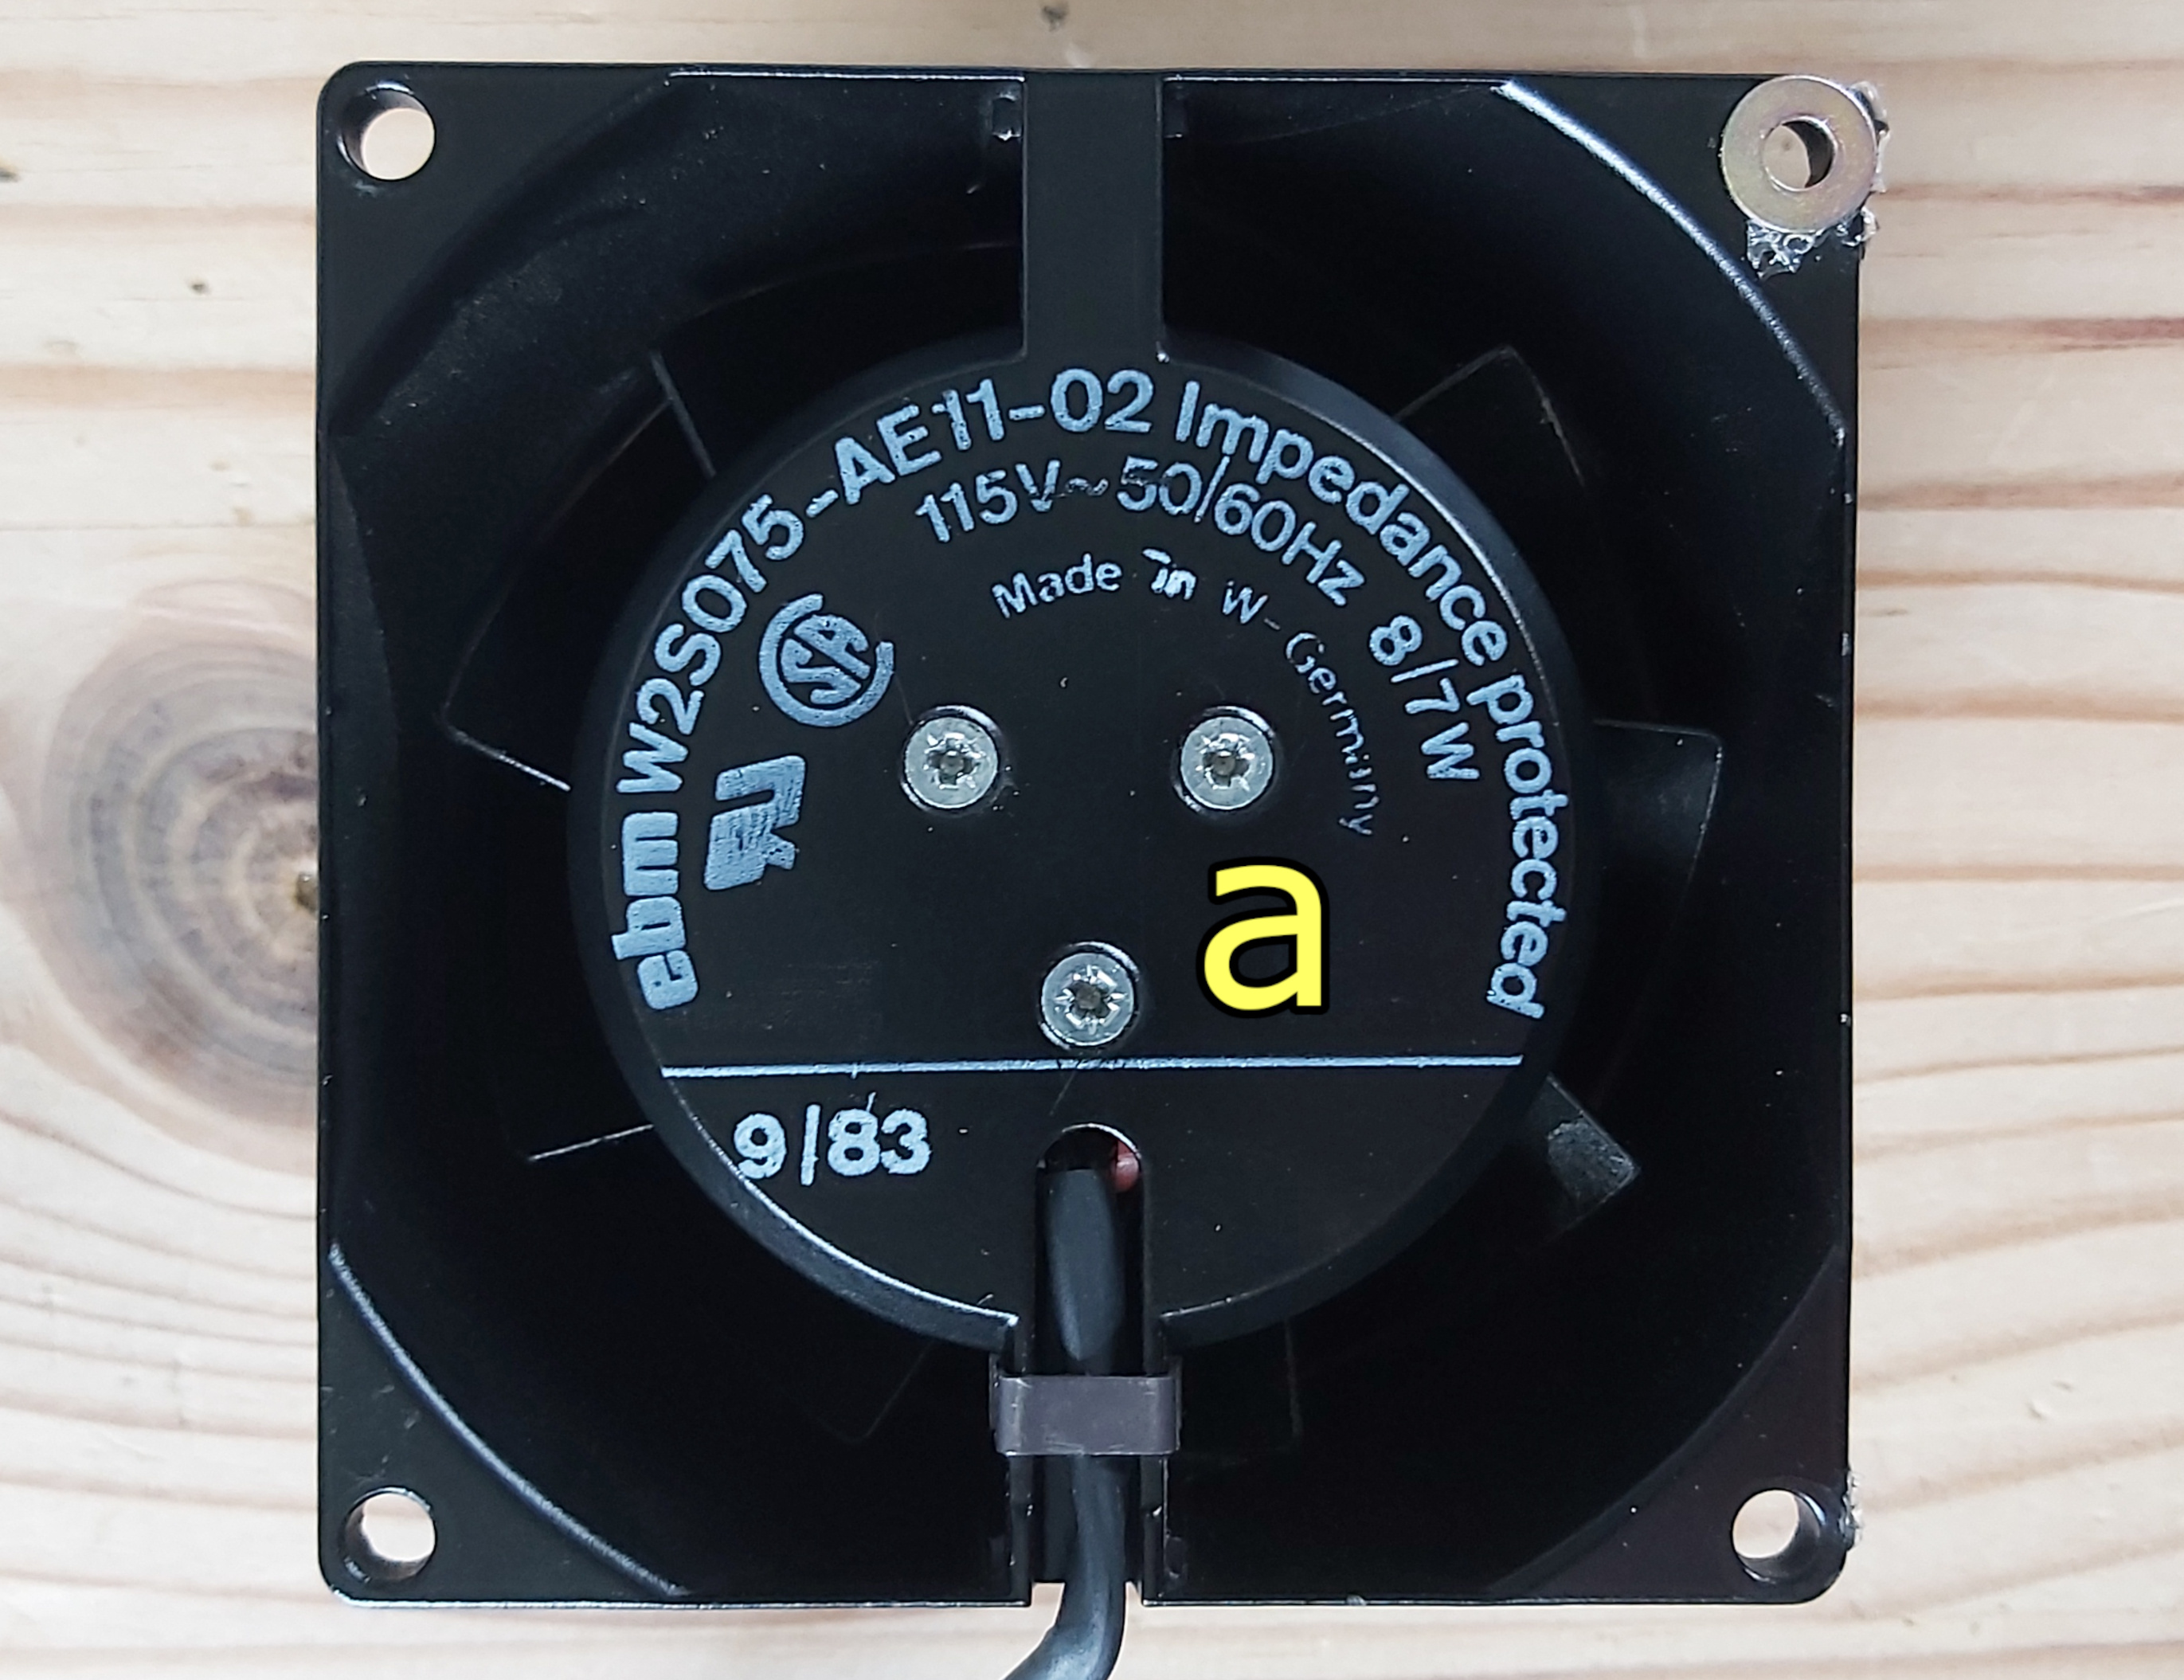
\includegraphics[width=\columnwidth]{images/fan-image-1.jpg}
	\caption[Fan blade assembly screws]{Adjust the blade assembly screws.}
	\label{fig:fanassembly}
\end{figure}

\cleardoublepage
\twocolumn[\begin{@twocolumnfalse}
	\chapter{Making a Keyboard Adaptor cable\hfill\difficulty{3}}
	 Some `New Old Stock' (NOS) NABU Personal Computers are being sold without keyboards. Keyboards for other NABU PCs have over the years been misplaced or have developed faults. To address these issues, the NABU Preservation Project has released a Keyboard Emulator\footnotemark. The Keyboard Emulator software, in combination with a USB to RS-422 interface and a keyboard adaptor cable, allows NABU systems without keyboards to be controlled from a Windows PC. This section describes how to create the required DB-9 to DIN-6 keyboard adaptor cable.
	\vskip1em
\end{@twocolumnfalse}]
\footnotetext[1]{See the NABU RetroNet website <https://nabu.ca> for details.}

\section{Keyboard Adaptor cable wiring}
The \texttt{KEYBOARD} port on the back of the NABU Personal Computer implements a half-duplex RS-422 interface, which requires 2 wires for communication between devices. The cable must be connected as specified in Table~\ref{tbl:kbdadaptor}. For best performance, the adaptor cable should be kept as short as possible --- preferably less than 6 inches. Twisted-pair cable is highly recommended. To avoid a ground loop, only connect ground to either the DB-9 or DIN-6 connector, \textit{never both}.

\begin{center}
	\sffamily
	\begin{tblr}{
			colspec={r|cccc|},
			cell{1}{2} = {c=2}{c},
			cell{1}{4} = {c=2}{c},
			row{1} = {font=\bfseries},
			row{1,2} = {bg=gray4,fg=white},
			row{5,6} = {bg=gray9},
			cell{1}{1} = {r=2}{bg=white},
			cell{3}{1} = {r=2}{},
			cell{5}{1} = {r=2}{},
			vline{4} = {3-4}{text=\clap{$\leftrightarrow$}},
			vline{1} = {3-4}{solid},
			hline{1} = {2-5}{solid},
			hline{3,5} = {solid}
		}
		& NABU (DIN6) & & RS-422 (DB9)\footnotemark[2] &\\
		& Signal & Pin & Pin & Signal \\
		\rotatebox{90}{Pair} & T/R+ & 4 & 1 & T/R+ \\
		& T/R-- & 5 & 2 & T/R-- \\
	\end{tblr}
	\taskLbl{tbl:kbdadaptor}
	\taskTable{Adaptor cable wiring.}
\end{center}
\footnotetext[2]{Pin numbers shown are for the DTECH DT-5019 USB TO RS485/422 adaptor cable.  Refer to the relevant manufacturer's documentation for other RS-422 interfaces.}

\section{DIN-6 end of the cable}
\begin{enumerate}
	\item Solder the pins of a \underline{male} DIN-6 connector as shown in Figure \ref{fig:din6}. Note that the pin numbers shown in the diagram are for the solder side of the connector.
\end{enumerate}

\section{DB-9 end of the cable}
\begin{enumerate}
	\item Solder the pins on the \underline{female} DB-9 connector as shown in Figure \ref{fig:db9-kbd}.  Note that the pin numbers shown in the diagram are for the solder side of the connector.\\
	Alternatively, use a DB-9 adaptor with screw terminals, as shown in Figure \ref{fig:db9adapt-kbd}.
\end{enumerate}
\newpage
\begin{figure}[h!]
	\begin{center}
		\scalebox{0.175}{
			\begin{tikzpicture}[font=\sffamily]
				\draw[line width=6mm] (40,19) -- ++(-40,0) -- ++(0,-19) -- ++(40,0);
				\draw[line width=1mm,decorate,decoration={saw,segment length=45mm,amplitude=10mm}] (40,0) -- ++(0,19);
				\draw[line width=2mm,fill=white] (3,8) rectangle (18,16);
				\draw[line width=2mm,fill=white] (21,8) rectangle (36,16);
				\draw[line width=1mm,fill=white] (2.5,12) circle (4mm);
				\draw[line width=1mm,fill=white] (18.5,12) circle (4mm);
				\draw[line width=1mm,fill=white] (20.5,12) circle (4mm);
				\draw[line width=1mm,fill=white] (36.5,12) circle (4mm);

				\draw[line width=2mm,fill=white] (7,5) circle (15mm);
				\draw[line width=2mm,color=red,fill=white] (32,5) circle (15mm);
				\node[black,scale=4] at (7,2) {ADAPTOR};
				\node[black,scale=4] at (32,2) {KEYBOARD};
				\draw[line width=2mm,fill=white] (16,3.7) rectangle (22,5.5); \node[black,scale=4,] at (19,2) {PRINTER};
			\end{tikzpicture}
		}
		\caption[Keyboard port position.]{NABU Personal Computer \texttt{KEYBOARD} port.}
		\label{fig:backkbd}
	\end{center}
\end{figure}

\begin{figure}[h!]
	\begin{center}
		\scalebox{0.175}{
			\begin{tikzpicture}[font=\sffamily]
				\draw[line width=6mm] (10,10) circle (8cm);
				\draw[line width=1mm] (10,10) circle (7cm);
				\fill[fill=white] (9,3.5) rectangle (11,2.8);
				\begin{scope}
					\clip (8.8,3.05) rectangle (11.2,6);
					\draw[line width=1mm] (10,3) circle (1cm);
				\end{scope}
				\foreach \p\k\m\n [count=\q from 1] in {
					{}/1/6.6/8.1,{}/2/6.6/12.1,{}/6/10/10,
					{}/3/10/14,{T/R--}/5/13.4/8.1,{T/R+}/4/13.4/12.1}
				{
					\ifthenelse{\q>4}{
						\pgfmathsetmacro{\r}{\q*30+-165}
						\draw[line width=1mm,red] (\m,\n) -- ++(\r:6cm) node[black,scale=4,text width=2.2cm,align=right]{\p};
					}{}
					\draw[line width=1mm,fill=white] (\m,\n) circle (7mm) node[scale=3,gray,yshift=-1.5em]{\k};
				}
			\end{tikzpicture}
		}
		\caption[DIN-6 male connector pinouts.]{DIN-6 male connector (solder side).}
		\label{fig:din6}
	\end{center}
\end{figure}

\begin{figure}[h!]
  \begin{center}
	\scalebox{0.2}{
		\begin{tikzpicture}[font=\sffamily]
			\draw[rounded corners=2cm,line width=6mm] (0, 0) rectangle (25,10) {};

			\draw[line width=4mm] (3,5) circle (1.4cm);
			\draw[line width=4mm] (22,5) circle (1.4cm);

			\draw[line width=1mm] (7,8) -- (18,8);
			\draw[line width=1mm] (8,2) -- (17,2);
			\draw[line width=1mm] (6,7) -- (7,3);
			\draw[line width=1mm] (19,7) -- (18,3);
			\draw[line width=1mm] (6,7) to[out=102,in=180,distance=22] (7,8);
			\draw[line width=1mm] (7,3) to[out=-78,in=180,distance=22] (8,2);
			\draw[line width=1mm] (17,2) to[out=0,in=-102,distance=22] (18,3);
			\draw[line width=1mm] (19,7) to[out=78,in=0,distance=22] (18,8);

			\draw[line width=1mm] (7,8.5) -- (18,8.5);
			\draw[line width=1mm] (8,1.5) -- (17,1.5);
			\draw[line width=1mm] (5.5,7) -- (6.5,3);
			\draw[line width=1mm] (19.5,7) -- (18.5,3);
			\draw[line width=1mm] (5.5,7) to[out=102,in=180,distance=30] (7,8.5);
			\draw[line width=1mm] (6.5,3) to[out=-78,in=180,distance=30] (8,1.5);
			\draw[line width=1mm] (17,1.5) to[out=0,in=-102,distance=30] (18.5,3);
			\draw[line width=1mm] (19.5,7) to[out=78,in=0,distance=30] (18,8.5);

			\foreach \p\k [count=\q from 0] in {{T/R+}/{},{T/R--}/{},{}/{},{}/{},{}/{}} {
				\draw[line width=1mm] (8.4+\q*2,6.2) circle (4mm);
				\ifthenelse{\q<4}{\draw[line width=1mm] (9.4+\q*2,3.8) circle (4mm);	}{}
				\foreach \x in \p {
					\draw[line width=1mm,red] (8.4+\q*2,6.6) -- ++(0,6);
					\draw (8.4+\q*2,14.8) node[rotate=-90,scale=4]{\p};
				}{}
				\foreach \x in \k {
					\draw[line width=1mm,red] (9.4+\q*2,3.4) -- ++(0,-6);
					\draw (9.4+\q*2,-4.8) node[rotate=-90,scale=4,text width=1cm]{\k};
				}
				\draw (7.4,6.6) node[scale=3,gray]{1};
				\draw (17.45,6.6) node[scale=3,gray]{5};
				\draw (8.4,3.4) node[scale=3,gray]{6};
				\draw (16.45,3.4) node[scale=3,gray]{9};
			}
		\end{tikzpicture}
	}
	\caption[DB-9 female connector pinouts.]{DB-9 female connector (solder side).$^2$}
	\label{fig:db9-kbd}
  \end{center}
\end{figure}

\begin{figure}[h!]
	\begin{center}
		\scalebox{0.19}{
			\begin{tikzpicture}[font=\sffamily]
				\draw[] (2,0) rectangle (12.3,16);
				\draw[] (10,2) rectangle (12,14);
				\draw[line width=4mm, color=red] (22.9,4) -- (25,4) node [scale=4,xshift=3.2em,text width=2cm] {5 T/R--};
				\draw[line width=4mm, color=red] (11,6) -- (14,6);
				\draw[line width=4mm, color=blue] (22.9,6) -- (25,6)  node [scale=4,xshift=3.2em,text width=2cm] {4 T/R+};
				\draw[line width=4mm, color=blue] (11,4) -- (14,4);
				\draw[fill=black!40] (0,4) rectangle (2,12);
				\foreach \k [count=\q from 0] in {{T/R+},{T/R--},{RXD+},{RXD--},{GND}}{
					\draw[line width=1mm,fill=white] (11,\q*2+4) circle (5mm);
					\draw[line width=1mm] (11.5,\q*2+4) -- ++(-1,0) node [scale=4,xshift=-.5em,text width=2cm, align=left] {\k};
				}
				\draw[fill=black!40] (35,3) rectangle (39,7);
				\draw[] (25,2.5) rectangle (35,7.5);

				\begin{scope}
					\clip(14,2) rectangle (22.9,7);
					\draw[line width=4mm,color=blue,decorate,decoration={coil,aspect=0, amplitude=10mm,segment length=20mm}] (12.5,5) -- (23.6,5);
					\draw[line width=4mm,color=red,decorate,decoration={coil,aspect=0, amplitude=10mm,segment length=20mm}] (23.5,5) -- (12.2,5);
				\end{scope}
			\end{tikzpicture}
		}
	\caption[DB-9 adaptor terminals.]{DB-9 adaptor to DIN-6 wiring.$^2$}
	\label{fig:db9adapt-kbd}
	\end{center}
\end{figure}

\cleardoublepage
\twocolumn[\begin{@twocolumnfalse}
	\chapter{Making a Network Adaptor cable\hfill\difficulty{3}}
	The NABU Network Adaptor is the interface between the NABU Personal Computer and the cable television network that enables software applications and other digital data to be downloaded from NABU's back-end systems. The NABU Preservation Project has released an Internet Adaptor\footnotemark, which emulates the NABU Network Adaptor, allowing a NABU PC to download applications and data via the Internet. This section describes how to create a DB-9 to DIN-5 adaptor cable that allows a NABU PC to be connected via RS-422 to a system running the Internet Adaptor software. If required, a RS-422 interface can easily be added to the system hosting the Internet Adapter by means of a USB to RS-422 adaptor.
	\vskip1em
\end{@twocolumnfalse}]
\footnotetext[1]{See the NABU RetroNet website <https://nabu.ca> for details.}

\section{Network Adaptor cable wiring}
The \texttt{ADAPTOR} port on the back of the NABU Personal Computer implements a full-duplex RS-422 interface, which requires 4 wires for communication between devices. Because of the high transmission (baud) rates involved, a twisted-pair shielded cable is highly recommended for the DB-9 to DIN-5 adaptor (as per the RS-422 standard). Category 5 cable (as used in Ethernet cabling) is available both as shielded twisted pair and as unshielded twisted pair and generally exceeds the recommendations for RS-422, making it an excellent choice --- if no twisted pair cable is available, the length of the adaptor cable \textit{must} be kept as short as possible, and should not exceed 6-8 inches. When using shielded cable, the shielding must only be connected to one of the connectors to avoid a ground loop.

The cable must be wired as specified in Table~\ref{tbl:adaptor}. If at all possible, use twisted-pair cable and group the pairs as shown.

\begin{center}
	\sffamily
	\begin{tblr}{
			colspec={r|cccc|},
			cell{1}{2} = {c=2}{c},
			cell{1}{4} = {c=2}{c},
			row{1} = {font=\bfseries},
			row{1,2} = {bg=gray4,fg=white},
			row{5,6} = {bg=gray9},
			cell{1}{1} = {r=2}{bg=white},
			cell{3}{1} = {r=2}{},
			cell{5}{1} = {r=2}{},
			vline{4} = {3-6}{text=\clap{$\leftrightarrow$}},
			vline{1} = {3-6}{solid},
			hline{1} = {2-5}{solid},
			hline{3,7} = {solid}
		}
		& NABU (DIN5) & & RS-422 (DB9)\footnotemark[2] &\\
		& Signal & Pin & Pin & Signal \\
		\rotatebox{90}{Pair 1} & RXD+ & 1 & 1 & T/R+ \\
		& RXD-- & 4 & 2 & T/R-- \\
		\rotatebox{90}{Pair 2} & T/R+ & 5 & 3 & RXD+ \\
		& T/R-- & 3 & 4 & RXD-- \\
	\end{tblr}
	\captionof{table}{Adaptor cable wiring.}
	\label{tbl:adaptor}
\end{center}
\footnotetext[2]{Pin numbers shown are for the DTECH DT-5019 USB TO RS485/422 adaptor cable.  Refer to the relevant manufacturer's documentation for other RS-422 interfaces.}

\section{DIN-5 end of the cable}
\awesomebox[red]{2pt}{\faHandPaper}{red}{To avoid a ground loop, the cable shield should only ever be connected to ground at one end of the cable; \textit{never} at both ends. Thus, if the cable shield is connected to ground at the \mbox{RS-422} adaptor end, do \textit{not} also connect the shield to the outer rim of the DIN connector, or vice versa.}
\begin{enumerate}
	\item To minimise the number of connections that need to be soldered, a MIDI cable may be used. Alternatively, solder the pins of a \underline{male} DIN-5 connector as shown in Figure \ref{fig:din5}. Note that the pin numbers shown in the diagram are for the solder side of the connector. Also note that the \mbox{DIN-5} connector pins are not numbered sequentially.
\end{enumerate}

\begin{figure}[t!]
	\begin{center}
		\scalebox{0.175}{
			\begin{tikzpicture}[font=\sffamily]
				\draw[line width=6mm] (40,19) -- ++(-40,0) -- ++(0,-19) -- ++(40,0);
				\draw[line width=1mm,decorate,decoration={saw,segment length=45mm,amplitude=10mm}] (40,0) -- ++(0,19);
				\draw[line width=2mm,fill=white] (3,8) rectangle (18,16);
				\draw[line width=2mm,fill=white] (21,8) rectangle (36,16);
				\draw[line width=1mm,fill=white] (2.5,12) circle (4mm);
				\draw[line width=1mm,fill=white] (18.5,12) circle (4mm);
				\draw[line width=1mm,fill=white] (20.5,12) circle (4mm);
				\draw[line width=1mm,fill=white] (36.5,12) circle (4mm);

				\draw[line width=2mm,color=red,fill=white] (7,5) circle (15mm);
				\draw[line width=2mm,fill=white] (32,5) circle (15mm);
				\node[black,scale=4] at (7,2) {ADAPTOR};
				\node[black,scale=4] at (32,2) {KEYBOARD};
				\draw[line width=2mm,fill=white] (16,3.7) rectangle (22,5.5); \node[black,scale=4,] at (19,2) {PRINTER};
			\end{tikzpicture}
		}
		\caption[Adaptor port position.]{NABU Personal Computer \texttt{ADAPTOR} port.}
		\label{fig:backplane}
	\end{center}
\end{figure}

\begin{figure}[h!]
	\begin{center}
		\scalebox{0.175}{
			\begin{tikzpicture}[font=\sffamily]
				\draw[line width=6mm] (10,10) circle (8cm);
				\draw[line width=1mm] (10,10) circle (7cm);
				\fill[fill=white] (9,3.5) rectangle (11,2.8);
				\begin{scope}
					\clip (8.8,3.05) rectangle (11.2,6);
					\draw[line width=1mm] (10,3) circle (1cm);
				\end{scope}
				\foreach \p\k\n\m\r [count=\q from 0] in {{RXD+}/1/10/5/190,{RXD--}/4/13.4/6.4/160,{}/2/15/10/0,{T/R+}/5/13.4/13.6/20,{T/R--}/3/10/15/350} {
					\ifthenelse{\k=2}{}{
						\ifthenelse{\q>1}{\def\a{right}\def\w{1.75cm}}{\def\a{left}\def\w{2.25cm}}
						\draw[line width=1mm,red] (\m,\n) -- ++(\r:6cm) node[black,scale=4,text width=\w,align=\a]{\p};
					}
					\draw[line width=1mm,fill=white] (\m,\n) circle (7mm) node[scale=3,gray,yshift=-1.5em]{\k};
				}
			\end{tikzpicture}
		}
		\caption[DIN-5 male connector pinouts.]{DIN-5 male connector (solder side).}
		\label{fig:din5}
	\end{center}
\end{figure}

\section{DB-9 end of the cable}
\begin{enumerate}
	\item Solder the pins on the \underline{female} DB-9 connector as shown in Figure \ref{fig:dsub9}.  Note that the pin numbers shown in the diagram are for the solder side of the connector.
\end{enumerate}

\begin{figure}[h!]
  \begin{center}
	\scalebox{0.2}{
		\begin{tikzpicture}[font=\sffamily]
			\draw[rounded corners=2cm,line width=6mm] (0, 0) rectangle (25,10) {};

			\draw[line width=4mm] (3,5) circle (1.4cm);
			\draw[line width=4mm] (22,5) circle (1.4cm);

			\draw[line width=1mm] (7,8) -- (18,8);
			\draw[line width=1mm] (8,2) -- (17,2);
			\draw[line width=1mm] (6,7) -- (7,3);
			\draw[line width=1mm] (19,7) -- (18,3);
			\draw[line width=1mm] (6,7) to[out=102,in=180,distance=22] (7,8);
			\draw[line width=1mm] (7,3) to[out=-78,in=180,distance=22] (8,2);
			\draw[line width=1mm] (17,2) to[out=0,in=-102,distance=22] (18,3);
			\draw[line width=1mm] (19,7) to[out=78,in=0,distance=22] (18,8);

			\draw[line width=1mm] (7,8.5) -- (18,8.5);
			\draw[line width=1mm] (8,1.5) -- (17,1.5);
			\draw[line width=1mm] (5.5,7) -- (6.5,3);
			\draw[line width=1mm] (19.5,7) -- (18.5,3);
			\draw[line width=1mm] (5.5,7) to[out=102,in=180,distance=30] (7,8.5);
			\draw[line width=1mm] (6.5,3) to[out=-78,in=180,distance=30] (8,1.5);
			\draw[line width=1mm] (17,1.5) to[out=0,in=-102,distance=30] (18.5,3);
			\draw[line width=1mm] (19.5,7) to[out=78,in=0,distance=30] (18,8.5);

			\foreach \p\k [count=\q from 0] in {{T/R+}/{},{T/R--}/{},{RXD+}/{},{RXD--}/{},{}/{}} {
				\fill[line width=1mm] (8.4+\q*2,6.2) circle (4mm);
				\ifthenelse{\q<4}{\fill[line width=1mm] (9.4+\q*2,3.8) circle (4mm);	}{}
				\foreach \x in \p {
					\draw[line width=1mm,red] (8.4+\q*2,6.6) -- ++(0,6);
					\draw (8.4+\q*2,14.8) node[rotate=-90,scale=4]{\p};
				}{}
				\foreach \x in \k {
					\draw[line width=1mm,red] (9.4+\q*2,3.4) -- ++(0,-6);
					\draw (9.4+\q*2,-4.8) node[rotate=-90,scale=4,text width=1cm]{\k};
				}
				\draw (7.4,6.6) node[scale=3,gray]{1};
				\draw (17.45,6.6) node[scale=3,gray]{5};
				\draw (8.4,3.4) node[scale=3,gray]{6};
				\draw (16.45,3.4) node[scale=3,gray]{9};
			}
		\end{tikzpicture}
	}
	\caption[DB-9 female connector pinouts.]{DB-9 female connector (solder side).$^2$}
	\label{fig:dsub9}
  \end{center}
\end{figure}
%\begin{figure}[t!]
%	\begin{center}
%		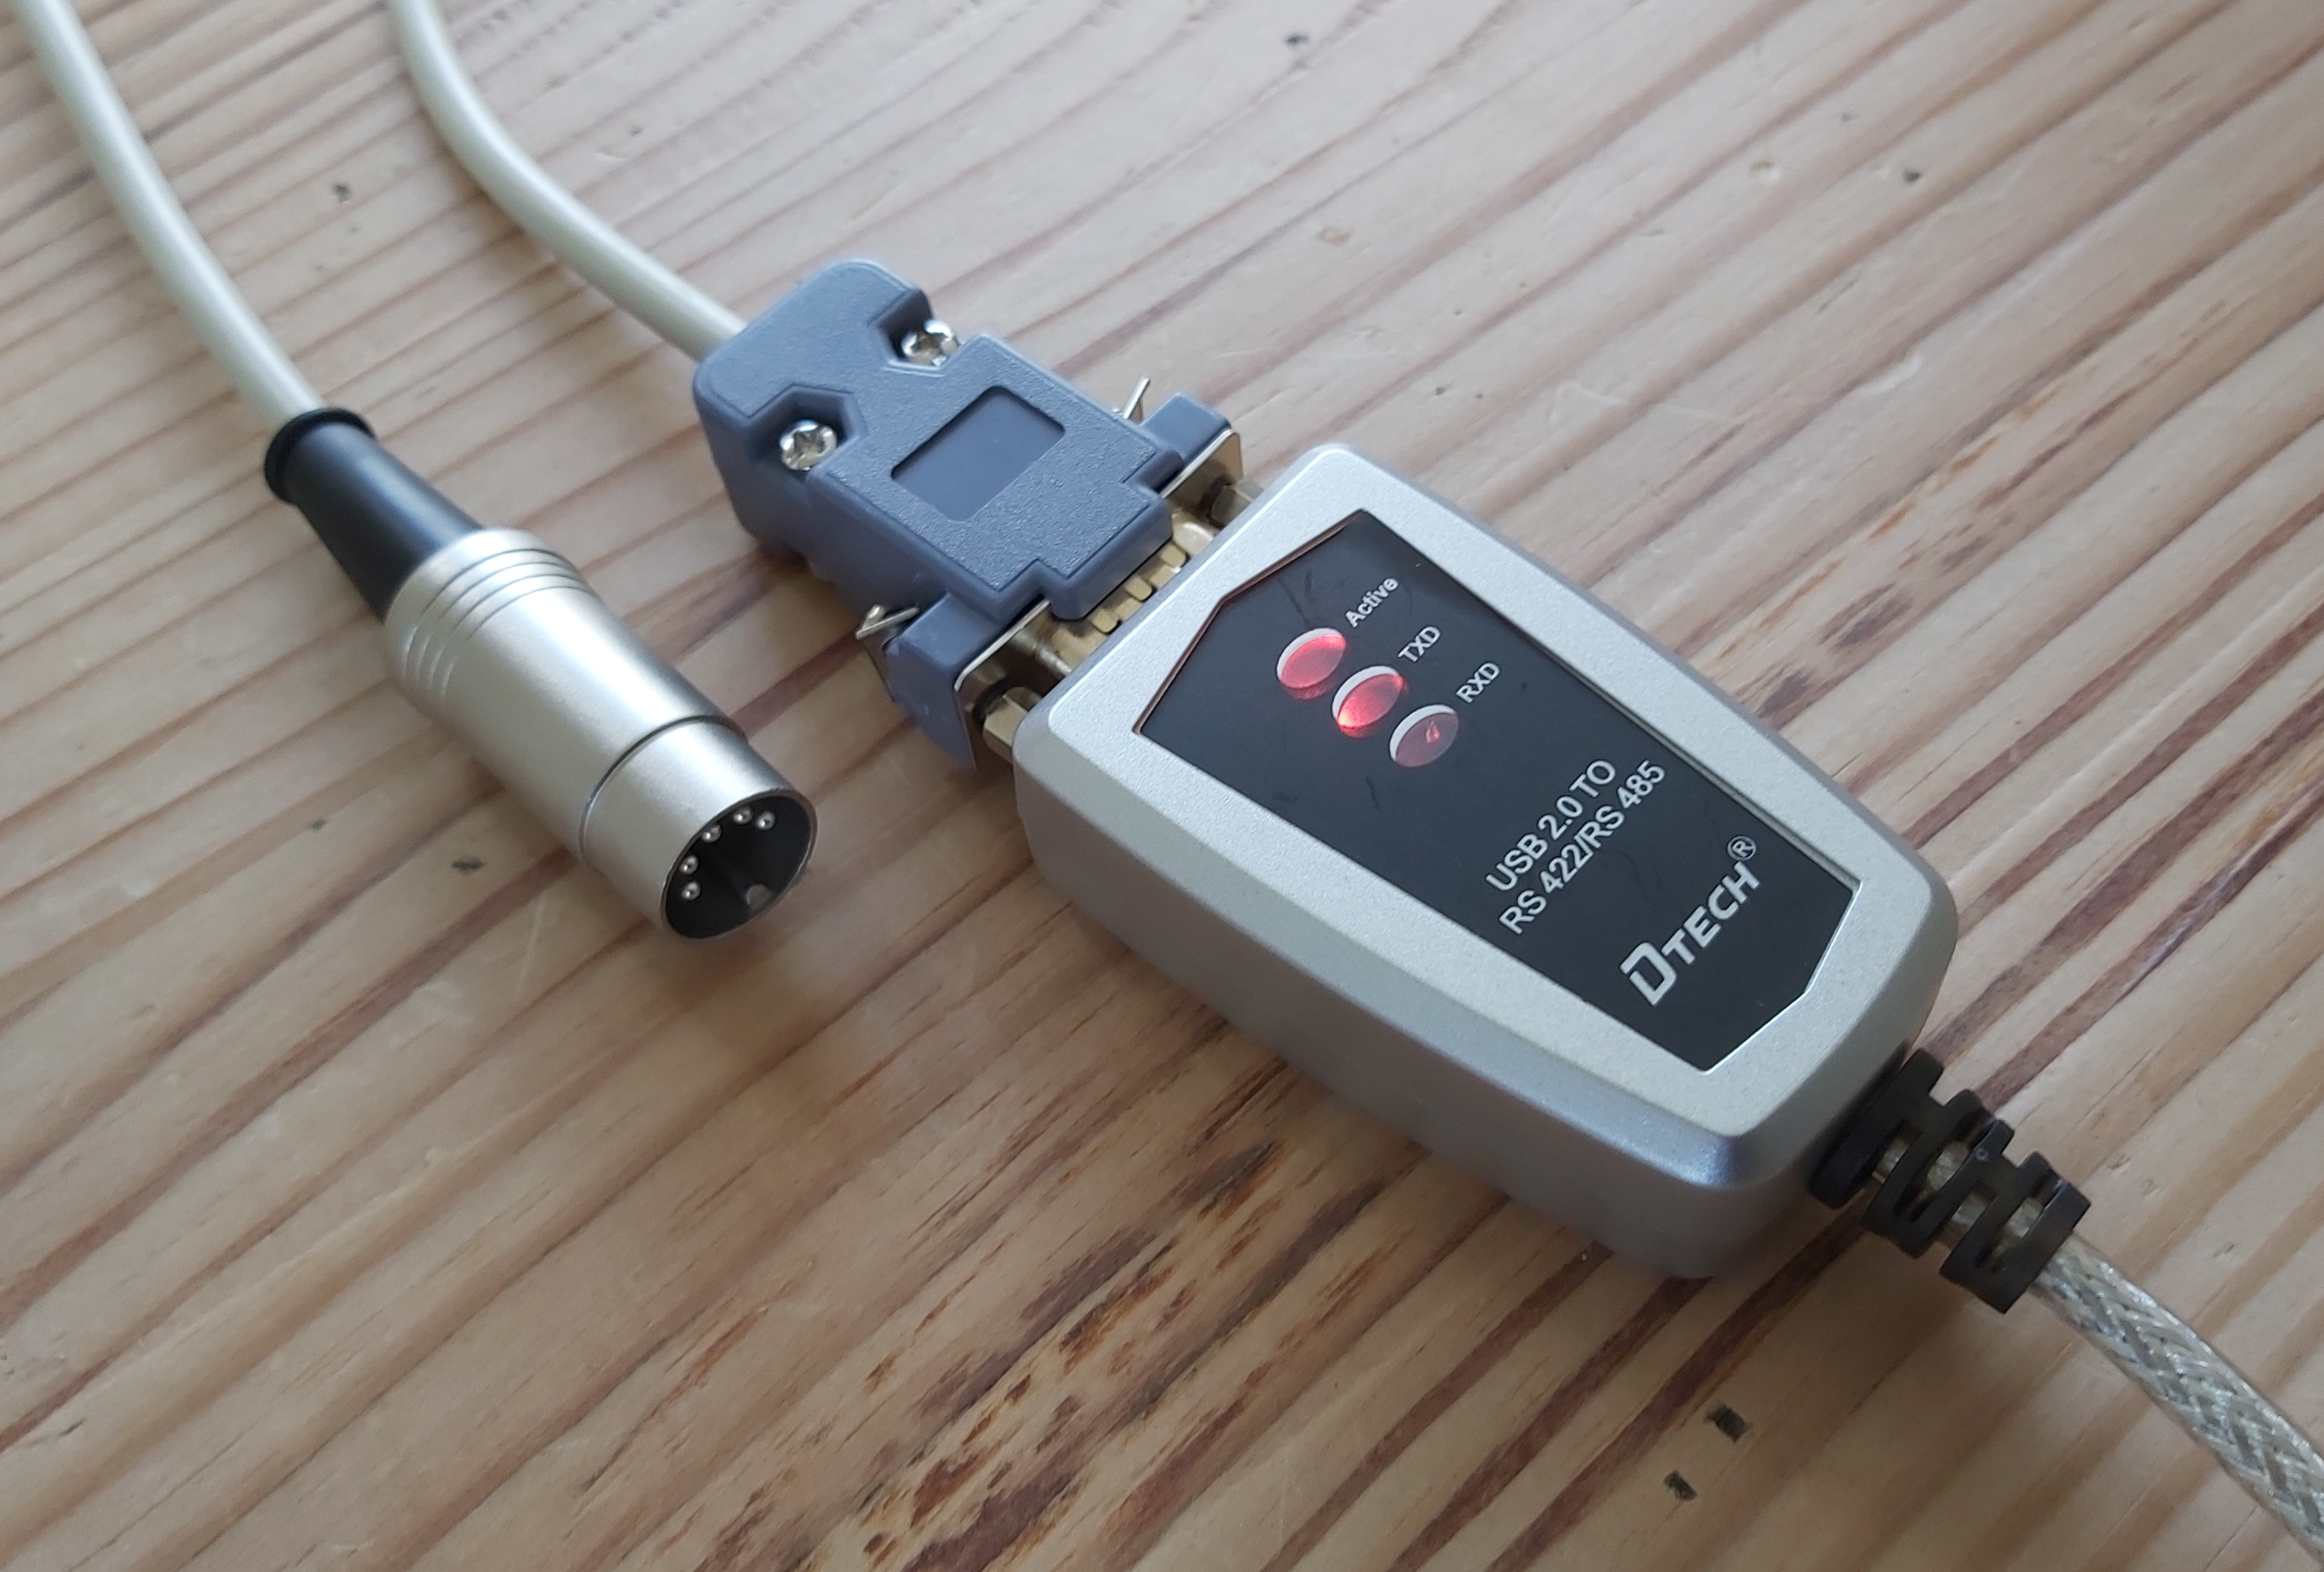
\includegraphics[width=\columnwidth]{images/rs422-image-1.jpg}
%		\caption{DB-9 to DIN-5 Network Adaptor assembly.}
%	\end{center}
%\end{figure}

\cleardoublepage
\twocolumn[\begin{@twocolumnfalse}
	\chapter{Making a Printer cable\hfill\difficulty{3}}
	 The NABU Personal Computer \texttt{PRINTER} port allows printers with Centronics (parallel) interfaces to be connected. Since the NABU port features a non-standard parallel port connector, either a custom cable or adaptor is required. This section describes both how to wire a cable with a DB-15 connector to a 36-way Centronics printer connector and how to make an adaptor, which allows `standard' printer cables to be used with the NABU.
	\vskip1em
\end{@twocolumnfalse}]

\section{NABU Printer cable wiring}
The \texttt{PRINTER} port on the back of the NABU Personal Computer implements a parallel interface. To make a printer cable use the wiring as specified in Table~\ref{tbl:prtcable}. For best performance, the cable should be shielded.

\begin{center}
	\sffamily
	\begin{tblr}{
			colspec={|cccc|},
			cell{1}{1} = {c=2}{c},
			cell{1}{3} = {c=2}{c},
			row{1} = {font=\bfseries},
			row{1,2} = {bg=gray4,fg=white},
			row{4,6,8,10,12} = {bg=gray9},
			vline{3} = {3-11}{text=\clap{$\rightarrow$}},
			vline{3} = {12-12}{text=\clap{$\leftarrow$}},
			vline{3} = {13-13}{text=\clap{--}},
%			vline{3} = {13-13}{text=\clap{$\leftrightarrow$}},
			hline{1,3,14} = {solid}
		}
		NABU (DB-15) & & Printer (Centronics) &\\
		Signal & Pin & Pin & Signal \\
		$\mathsf{\overline{Strobe}}$ & 1 & 1 & $\mathsf{\overline{Strobe}}$ \\
		Data 0 & 2 & 2 & Data 0 \\
		Data 1 & 3 & 3 & Data 1 \\
		Data 2 & 4 & 4 & Data 2 \\
		Data 3 & 5 & 5 & Data 3 \\
		Data 4 & 6 & 6 & Data 4 \\
		Data 5 & 7 & 7 & Data 5 \\
		Data 6 & 8 & 8 & Data 6 \\
		Data 7 & 9 & 9 & Data 7 \\
		$\mathsf{\overline{Busy}}$ & 11 & 11 & $\mathsf{\overline{Busy}}$ \\
		Ground & 15 & 16, 19--30 & Ground \\
	\end{tblr}
	\captionof{table}{Printer cable wiring.}
	\label{tbl:prtcable}
\end{center}

\section{NABU (DB-15) end of the cable}
\label{sec:db15}
\begin{enumerate}
	\item Solder the pins of the \underline{male double-row} DB-15 connector as shown in Figure \ref{fig:db15}. Note that the pin numbers shown in the diagram are for the solder side of the connector.
\end{enumerate}

\begin{figure}[h!]
	\begin{center}
		\scalebox{0.175}{
			\begin{tikzpicture}[font=\sffamily]
				\draw[rounded corners=2cm,line width=6mm] (0, 0) rectangle (31,10) {};

				\draw[line width=4mm] (3,5) circle (1.4cm);
				\draw[line width=4mm] (28,5) circle (1.4cm);

				\draw[line width=1mm] (7,8) -- (24,8);
				\draw[line width=1mm] (8,2) -- (23,2);
				\draw[line width=1mm] (6,7) -- (7,3);
				\draw[line width=1mm] (25,7) -- (24,3);
				\draw[line width=1mm] (6,7) to[out=102,in=180,distance=22] (7,8);
				\draw[line width=1mm] (7,3) to[out=-78,in=180,distance=22] (8,2);
				\draw[line width=1mm] (23,2) to[out=0,in=-102,distance=22] (24,3);
				\draw[line width=1mm] (25,7) to[out=78,in=0,distance=22] (24,8);

				\draw[line width=1mm] (7,8.5) -- (24,8.5);
				\draw[line width=1mm] (8,1.5) -- (23,1.5);
				\draw[line width=1mm] (5.5,7) -- (6.5,3);
				\draw[line width=1mm] (25.5,7) -- (24.5,3);
				\draw[line width=1mm] (5.5,7) to[out=102,in=180,distance=30] (7,8.5);
				\draw[line width=1mm] (6.5,3) to[out=-78,in=180,distance=30] (8,1.5);
				\draw[line width=1mm] (23,1.5) to[out=0,in=-102,distance=30] (24.5,3);
				\draw[line width=1mm] (25.5,7) to[out=78,in=0,distance=30] (24,8.5);

				\foreach \p\k [count=\q from 0] in {
					{Data~6}/{Ground},{Data~5}/{},{Data~4}/{},{Data~3}/{},{Data~2}/{$\mathsf{\overline{Busy}}$},{Data~1}/{},{Data~0}/{Data~7},{$\mathsf{\overline{Strobe}}$}/{}} {
					\draw[line width=1mm] (8.4+\q*2,6.2) circle (4mm);
					\ifthenelse{\q<7}{\draw[line width=1mm] (9.4+\q*2,3.8) circle (4mm);	}{}
					\foreach \x in \p {
						\draw[line width=1mm,red] (8.4+\q*2,6.6) -- ++(0,6);
						\draw (8.4+\q*2,14.8) node[rotate=-90,scale=4]{\p};
					}{}
					\foreach \x in \k {
						\draw[line width=1mm,red] (9.4+\q*2,3.4) -- ++(0,-6);
						\draw (9.4+\q*2,-4.8) node[rotate=-90,scale=4,text width=1cm]{\k};
					}
					\draw (7.4,6.6) node[scale=3,gray]{8};
					\draw (23.45,6.6) node[scale=3,gray]{1};
					\draw (8.4,3.4) node[scale=3,gray]{15};
					\draw (22.45,3.4) node[scale=3,gray]{9};
				}
		\end{tikzpicture}		}
		\caption[DB-15 male connector pinouts.]{DB-15 male connector (solder side).}
		\label{fig:db15}
	\end{center}
\end{figure}

\newpage

\begin{figure}[h!]
	\begin{center}
		\scalebox{0.175}{
			\begin{tikzpicture}[font=\sffamily]
				\draw[line width=6mm] (40,19) -- ++(-40,0) -- ++(0,-19) -- ++(40,0);
				\draw[line width=1mm,decorate,decoration={saw,segment length=45mm,amplitude=10mm}] (40,0) -- ++(0,19);
				\draw[line width=2mm,fill=white] (3,8) rectangle (18,16);
				\draw[line width=2mm,fill=white] (21,8) rectangle (36,16);
				\draw[line width=1mm,fill=white] (2.5,12) circle (4mm);
				\draw[line width=1mm,fill=white] (18.5,12) circle (4mm);
				\draw[line width=1mm,fill=white] (20.5,12) circle (4mm);
				\draw[line width=1mm,fill=white] (36.5,12) circle (4mm);

				\draw[line width=2mm,fill=white] (7,5) circle (15mm);
				\draw[line width=2mm,fill=white] (32,5) circle (15mm);
				\node[black,scale=4] at (7,2) {ADAPTOR};
				\node[black,scale=4] at (32,2) {KEYBOARD};
				\draw[line width=2mm,color=red,fill=white] (16,3.7) rectangle (22,5.5); \node[black,scale=4,] at (19,2) {PRINTER};
			\end{tikzpicture}
		}
		\caption[Printer port position.]{NABU Personal Computer \texttt{PRINTER} port.}
		\label{fig:backprt}
	\end{center}
\end{figure}

\section{Printer (Centronics) end of the cable}
\begin{enumerate}
	\item Solder the pins of the \underline{male} Centronics connector as shown in Figure \ref{fig:centronics}.  Note that the pin numbers shown in the diagram are for the solder side of the connector.\\
\end{enumerate}

\begin{figure}[h!]
	\begin{center}
		\scalebox{0.18}{
			\begin{tikzpicture}[font=\sffamily]
				\draw[rounded corners=1cm,line width=6mm] (.5, -.5) rectangle (34.5,10.5) {};

				\fill[color=black!80,line width=1mm] (-3,9.75) to[out=180,in=90] (-4,9) to[out=-90,in=135] (-3.5,8.25) -- (-2,6.75) to[out=-45,in=225] (-1.5,6.75) to[out=45,in=90,distance=22] (-0.5,6.75) -- (-0.5,3.25) to[out=-90,in=-45,distance=22] (-1.5,3.25) to [out=-225,in=45] (-2,3.25) -- (-3.5,1.75) to[in=90,out=-135] (-4,1) to[in=180,out=270] (-3,0.25) --
				(38,0.25) to [in=270,out=0] (39,1) to[in=135,out=90] (38.5,1.75) -- (37,3.25) to[in=45,out=135] (36.5,3.25) to[in=-90,out=-135,distance=22] (35.5,3.25) -- (35.5,6.75) to[in=135,out=90,distance=22] (36.5,6.75) to [in=-135,out=-45] (37,6.75) -- (38.5,8.25) to[in=-90,out=-135] (39,9) to[in=0,out=90] (38,9.75) -- cycle;

				\fill[line width=1mm,color=white] (3,8.5) -- (32,8.5) to[out=0,in=78,distance=30] (33.5,7) -- (32.5,3) to[in=0,out=-102,distance=30] (31,1.5) -- (4,1.5) to[in=-78,out=180,distance=30] (2.5,3) -- (1.5,7) to[out=102,in=180,distance=30] (3,8.5);

				\draw[line width=1mm] (3,8) -- (32,8);
				\draw[line width=1mm] (4,2) -- (31,2);
				\draw[line width=1mm] (2,7) -- (3,3);
				\draw[line width=1mm] (33,7) -- (32,3);
				\draw[line width=1mm] (2,7) to[out=102,in=180,distance=22] (3,8);
				\draw[line width=1mm] (3,3) to[out=-78,in=180,distance=22] (4,2);
				\draw[line width=1mm] (31,2) to[out=0,in=-102,distance=22] (32,3);
				\draw[line width=1mm] (33,7) to[out=78,in=0,distance=22] (32,8);

				\fill[fill=black!50] (4,3.7) rectangle (31,6.3);
				\foreach \x in {0,1,...,11} {
					\draw[line width=1mm,red] (13.7+\x*1.5,3.4) -- ++(0,-5.25);
				}
				\draw[line width=1mm,red] (9.2,-1.85) -- ++(21,0);
				\foreach \p\k [count=\q from 0] in {
					{}/{},{Shield}/{},{Ground}/{},{}/{Ground},{}/{},{}/{},{}/{},{$\mathsf{\overline{Busy}}$}/{},{}/{},{Data~7}/{},{Data~6}/{},{Data~5}/{},{Data~4}/{},{Data~3}/{},{Data~2}/{},{Data~1}/{},{Data~0}/{},{$\mathsf{\overline{Strobe}}$}/{}}{
					\foreach \x in \p {
						\draw[line width=1mm,red] (4.7+\q*1.5,6.6) -- ++(0,6);
						\draw (4.7+\q*1.5,14.8) node[rotate=-90,scale=4]{\p};
					}{}
					\foreach \x in \k {
						\draw[line width=1mm,red] (4.7+\q*1.5,3.4) -- ++(0,-6);
						\draw (4.7+\q*1.5,-4.8) node[rotate=-90,scale=4,text width=1cm]{\k};
					}
					\draw[line width=1mm,fill=white] (4.4+\q*1.5,5.5) rectangle (5+\q*1.5,7);
					\draw[line width=1mm,fill=white] (4.4+\q*1.5,4.5) rectangle (5+\q*1.5,3);
				}
				\draw (3.4,6.6) node[scale=3,gray]{18};
				\draw (31.45,6.6) node[scale=3,gray]{1};
				\draw (3.4,3.4) node[scale=3,gray]{36};
				\draw (31.45,3.4) node[scale=3,gray]{19};
			\end{tikzpicture}
		}
		\caption[Centronics male connector pinouts.]{Centronics male connector (solder side).}
		\label{fig:centronics}
	\end{center}
\end{figure}

\newpage

\section{NABU Printer Adaptor wiring}
To make an adaptor cable that allows the use of standard parallel printer cables use the wiring as specified in Table~\ref{tbl:prtadaptor}. The DB-15 connector (at the NABU end) should be wired as described in section \ref{sec:db15} on page \pageref{sec:db15}.

\begin{center}
	\sffamily
	\begin{tblr}{
			colspec={|cccc|},
			cell{1}{1} = {c=2}{c},
			cell{1}{3} = {c=2}{c},
			row{1} = {font=\bfseries},
			row{1,2} = {bg=gray4,fg=white},
			row{4,6,8,10,12} = {bg=gray9},
			vline{3} = {3-11}{text=\clap{$\rightarrow$}},
			vline{3} = {12-12}{text=\clap{$\leftarrow$}},
			vline{3} = {13-13}{text=\clap{--}},
			hline{1,3,14} = {solid}
		}
		NABU (DB-15) & & Adaptor (DB-25) &\\
		Signal & Pin & Pin & Signal \\
		$\mathsf{\overline{Strobe}}$ & 1 & 1 & $\mathsf{\overline{Strobe}}$ \\
		Data 0 & 2 & 2 & Data 0 \\
		Data 1 & 3 & 3 & Data 1 \\
		Data 2 & 4 & 4 & Data 2 \\
		Data 3 & 5 & 5 & Data 3 \\
		Data 4 & 6 & 6 & Data 4 \\
		Data 5 & 7 & 7 & Data 5 \\
		Data 6 & 8 & 8 & Data 6 \\
		Data 7 & 9 & 9 & Data 7 \\
		$\mathsf{\overline{Busy}}$ & 11 & 11 & $\mathsf{\overline{Busy}}$ \\
		Ground & 15 & 18--35 & Ground \\
	\end{tblr}
	\captionof{table}{Printer adaptor wiring.}
	\label{tbl:prtadaptor}
\end{center}

\section{Adaptor (DB-25) end of the cable}
\label{sec:db25}
\begin{enumerate}
	\item Solder the pins of a \underline{female} DB-25 connector as shown in Figure \ref{fig:db25}. Note that the pin numbers shown in the diagram are for the solder side of the connector.
\end{enumerate}

\begin{figure}[h!]
	\begin{center}
		\scalebox{0.175}{
			\begin{tikzpicture}[font=\sffamily]
				\draw[rounded corners=2cm,line width=6mm] (0, 0) rectangle (41,10) {};

				\draw[line width=4mm] (3,5) circle (1.4cm);
				\draw[line width=4mm] (38,5) circle (1.4cm);

				\draw[line width=1mm] (7,8) -- (34,8);
				\draw[line width=1mm] (8,2) -- (33,2);
				\draw[line width=1mm] (6,7) -- (7,3);
				\draw[line width=1mm] (35,7) -- (34,3);
				\draw[line width=1mm] (6,7) to[out=102,in=180,distance=22] (7,8);
				\draw[line width=1mm] (7,3) to[out=-78,in=180,distance=22] (8,2);
				\draw[line width=1mm] (33,2) to[out=0,in=-102,distance=22] (34,3);
				\draw[line width=1mm] (35,7) to[out=78,in=0,distance=22] (34,8);

				\draw[line width=1mm] (7,8.5) -- (34,8.5);
				\draw[line width=1mm] (8,1.5) -- (33,1.5);
				\draw[line width=1mm] (5.5,7) -- (6.5,3);
				\draw[line width=1mm] (35.5,7) -- (34.5,3);
				\draw[line width=1mm] (5.5,7) to[out=102,in=180,distance=30] (7,8.5);
				\draw[line width=1mm] (6.5,3) to[out=-78,in=180,distance=30] (8,1.5);
				\draw[line width=1mm] (33,1.5) to[out=0,in=-102,distance=30] (34.5,3);
				\draw[line width=1mm] (35.5,7) to[out=78,in=0,distance=30] (34,8.5);

				\foreach \p\k [count=\q from 0] in {
					{$\mathsf{\overline{Strobe}}$}/{},{Data~0}/{},{Data~1}/{},{Data~2}/{},{Data~3}/{Ground},{Data~4}/{},{Data~5}/{},{Data~6}/{},
					{Data~7}/{},{}/{},{$\mathsf{\overline{Busy}}$}/{},{}/{},{}/{}} {
					\fill[line width=1mm] (8.4+\q*2,6.2) circle (4mm);
					\ifthenelse{\q<12}{\fill[line width=1mm] (9.4+\q*2,3.8) circle (4mm);	}{}
					\foreach \x in \p {
						\draw[line width=1mm,red] (8.4+\q*2,6.6) -- ++(0,6);
						\draw (8.4+\q*2,14.8) node[rotate=-90,scale=4]{\p};
					}{}
					\foreach \x in \k {
						\draw[line width=1mm,red] (9.4+\q*2,3.4) -- ++(0,-6);
						\draw (9.4+\q*2,-4.8) node[rotate=-90,scale=4,text width=1cm]{\k};
					}
					\draw (7.4,6.6) node[scale=3,gray]{1};
					\draw (33.45,6.6) node[scale=3,gray]{13};
					\draw (8.4,3.4) node[scale=3,gray]{14};
					\draw (32.45,3.4) node[scale=3,gray]{25};
				}
				\foreach \x in {0,1,...,6} {
					\draw[line width=1mm,red] (19.4+\x*2,3.4) -- ++(0,-5.25);
				}
				\draw[line width=1mm,red] (17.4,-1.85) -- ++(14,0);
		\end{tikzpicture}
		}
		\caption[DB-25 female connector pinouts.]{DB-25 female connector (solder side).}
		\label{fig:db25}
	\end{center}
\end{figure}

\cleardoublepage
\twocolumn[\begin{@twocolumnfalse}
	\chapter{Replacing the NABU Power Supply\hfill\difficulty{4}}
	The NABU Personal Computer was developed for the North-American market, and as such, was fitted with a 110-120V power supply unit (PSU). The following section explains how to replace the NABU power supply with a modern, universal power supply.
	Note that the replacement PSU referred to in this guide is the Mean Well RT-65B. Refer to the relevant manufacturer's documentation for connection details when using other makes or models.
	\vskip1em
\end{@twocolumnfalse}]
\section{Removing the NABU PSU}
\awesomebox[red]{2pt}{\faBolt}{red}{To prevent electric shock, you \textbf{must} disconnect your NABU Personal Computer from mains power before removing the system cover!}
\begin{enumerate}
	\item Remove the outer computer cover by undoing the screws on either side of your NABU system. This will expose the main system board (right) and power supply bay (left).
	\item Remove the cover over the power supply by undoing the two screws on the right-hand side and lifting the cover upwards.
	\item Disconnect the motherboard (a), mains (b), and ground (c) connectors, as shown in Figure \ref{fig:connectors} below.
	\begin{figure}[b!]
		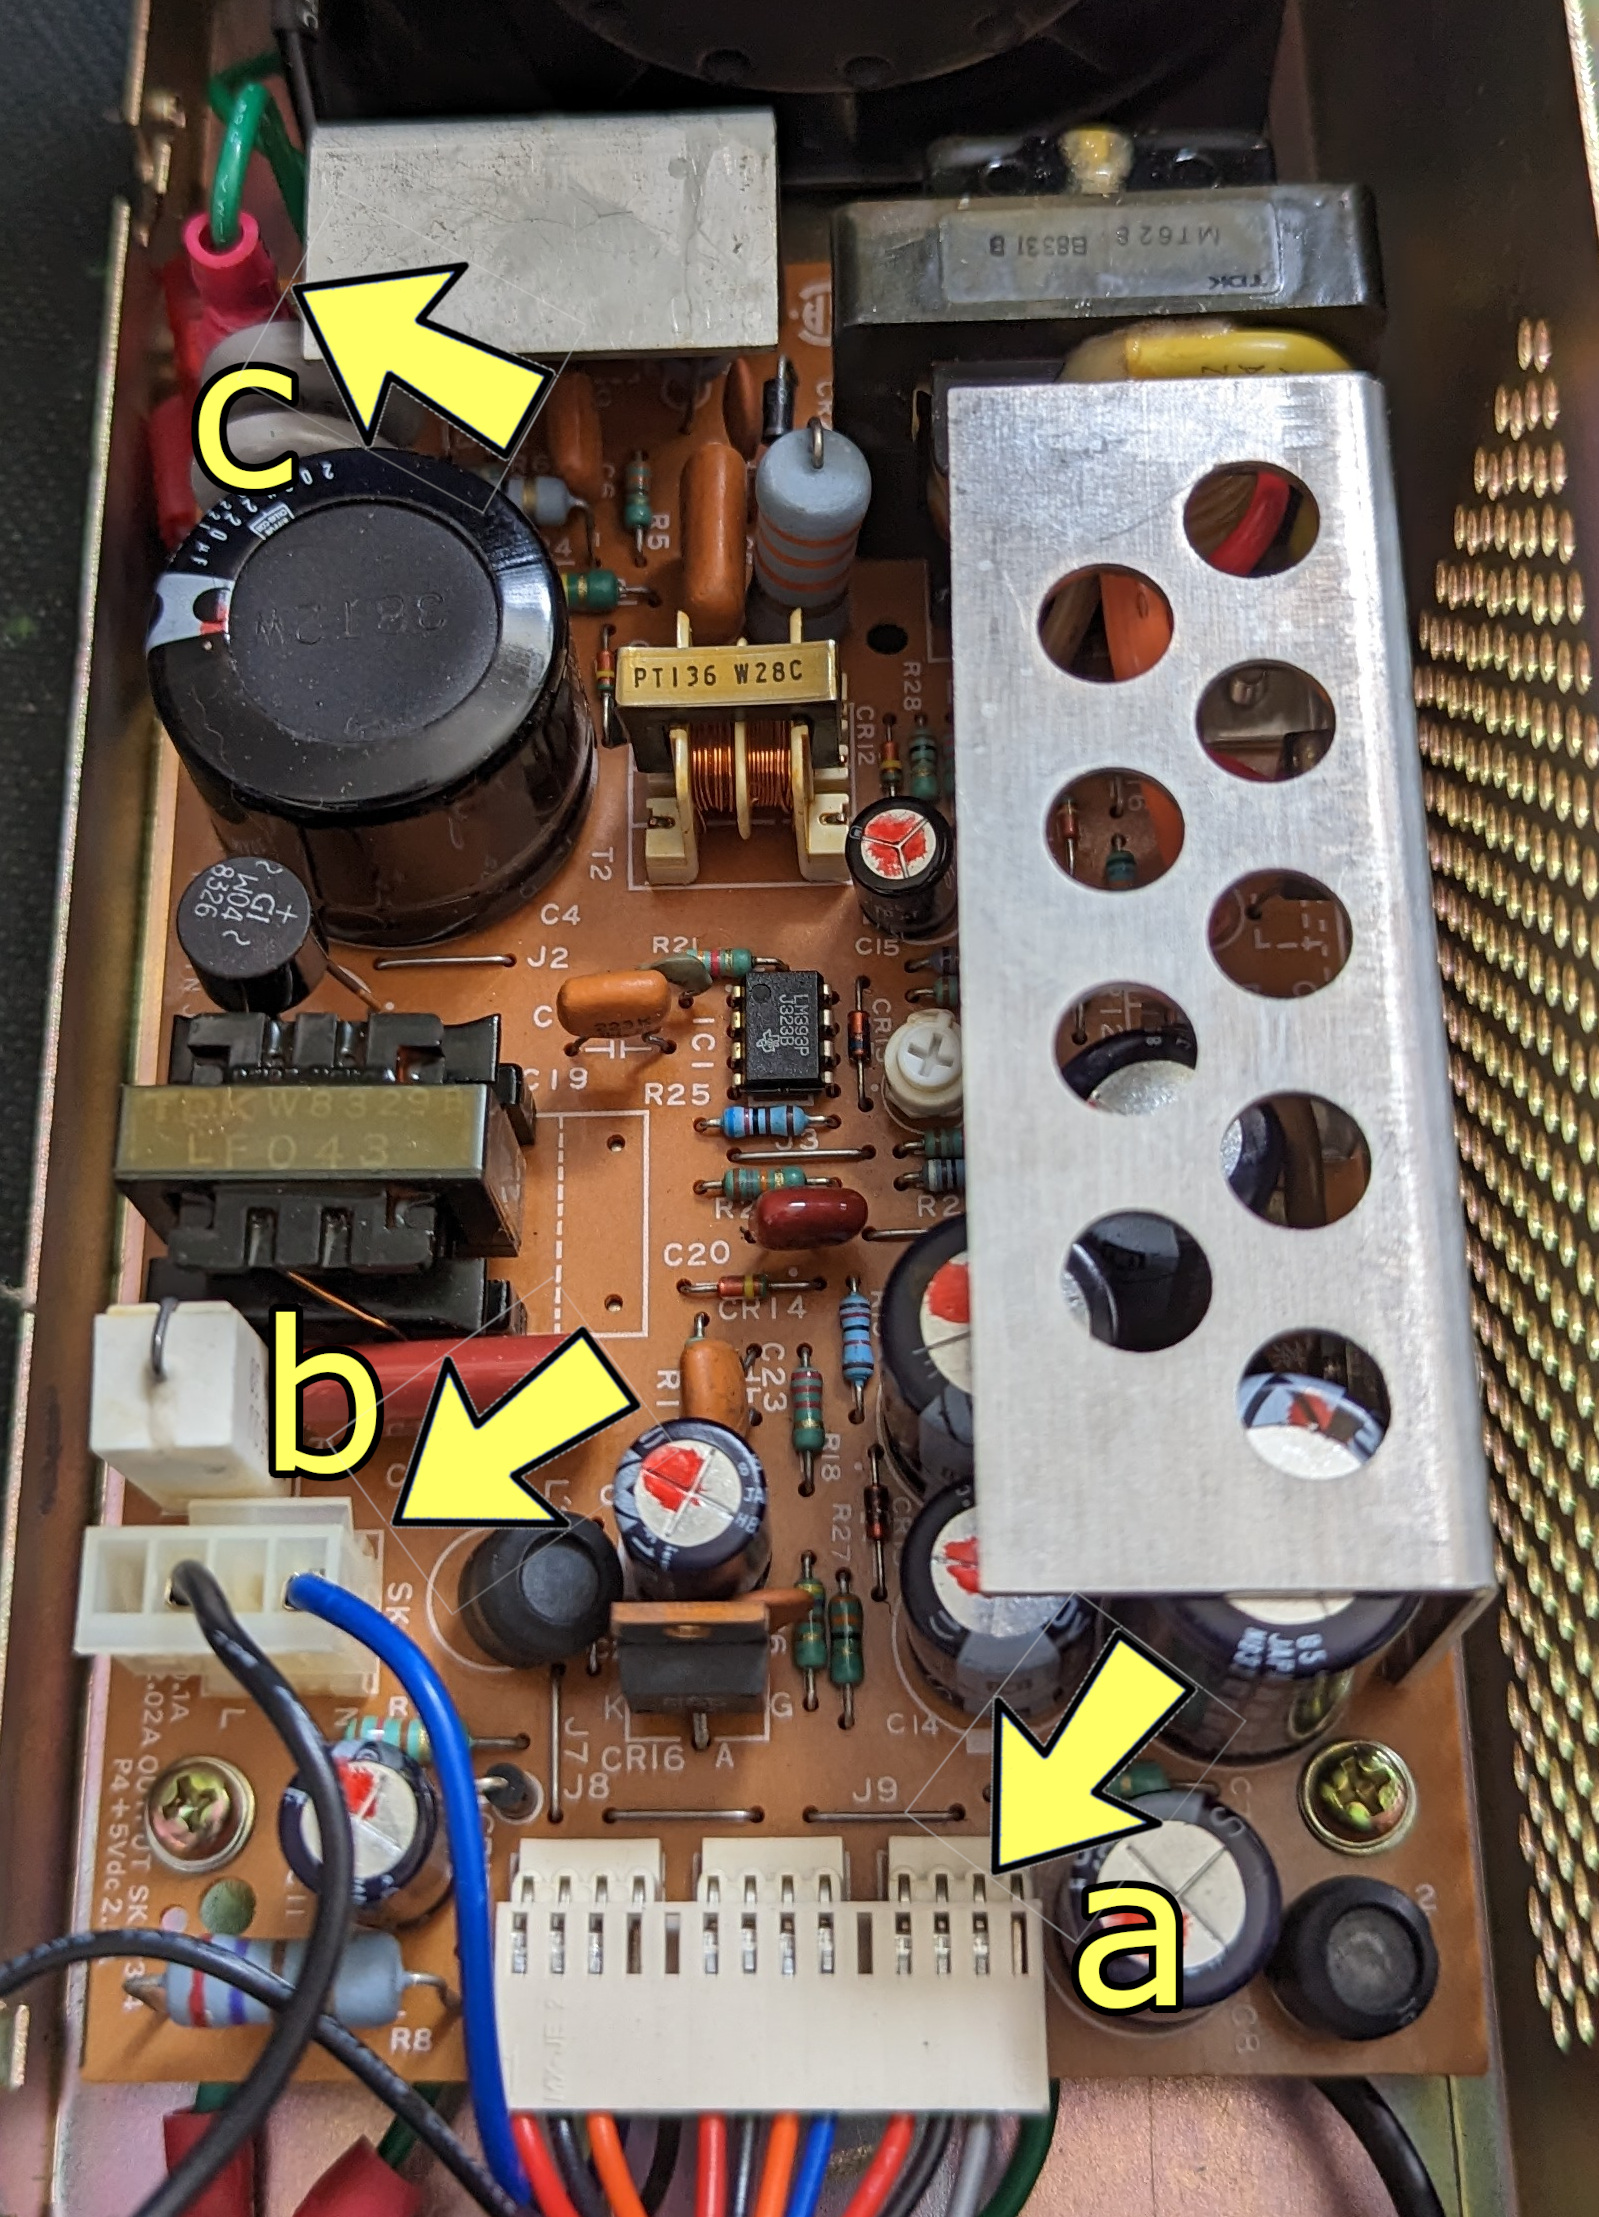
\includegraphics[width=\columnwidth]{images/psu-image-0.jpg}
		\caption{PSU connector positions.}
		\label{fig:connectors}
	\end{figure}
	\item Undo the 4 screws holding the PSU in place, and remove the PSU.
	\item Cut off both the motherboard (a) and mains (b) connectors as close as possible to each connector and strip a \textonequarter inch of insulation of the ends of all wires. Cut off the spade connector (c) and halve the length of the ground wire.
\end{enumerate}
\section{Replacing the NABU fan assembly}
\label{sec:fan-replacement}
As the fan fitted in the NABU power supply bay runs off 110-120V, it is no longer useful and should be removed. A suitable 80x80mm 12V or 5V fan may be fitted in its place.
\begin{enumerate}
	\item  To remove the fan, prise apart the crimp connector and cut the other lead near power button.
	\item Undo the 3 bolts which hold the assembly in place and remove the fan.
	\item Remove the remaining part of the fan power lead attached to the power button by gently removing the old heat shrink tubing and cutting the lead as close as possible to the terminal (see Figure \ref{fig:fan}). Then re-cover the terminal and remaining lead with a suitable length of new heat shrink tubing (as shown in Figure \ref{fig:tubing}).
	\item Remove the fan ground lead from the `ground post' by undoing the nut and lifting off the ring connector.
	\item Install the replacement fan using the bolts removed in the previous step, ensuring it is oriented such that air is sucked out of the NABU system. Guide the new fan leads towards the front of the system.
	\begin{figure}[h!]
		\begin{subfigure}[b]{\columnwidth}
			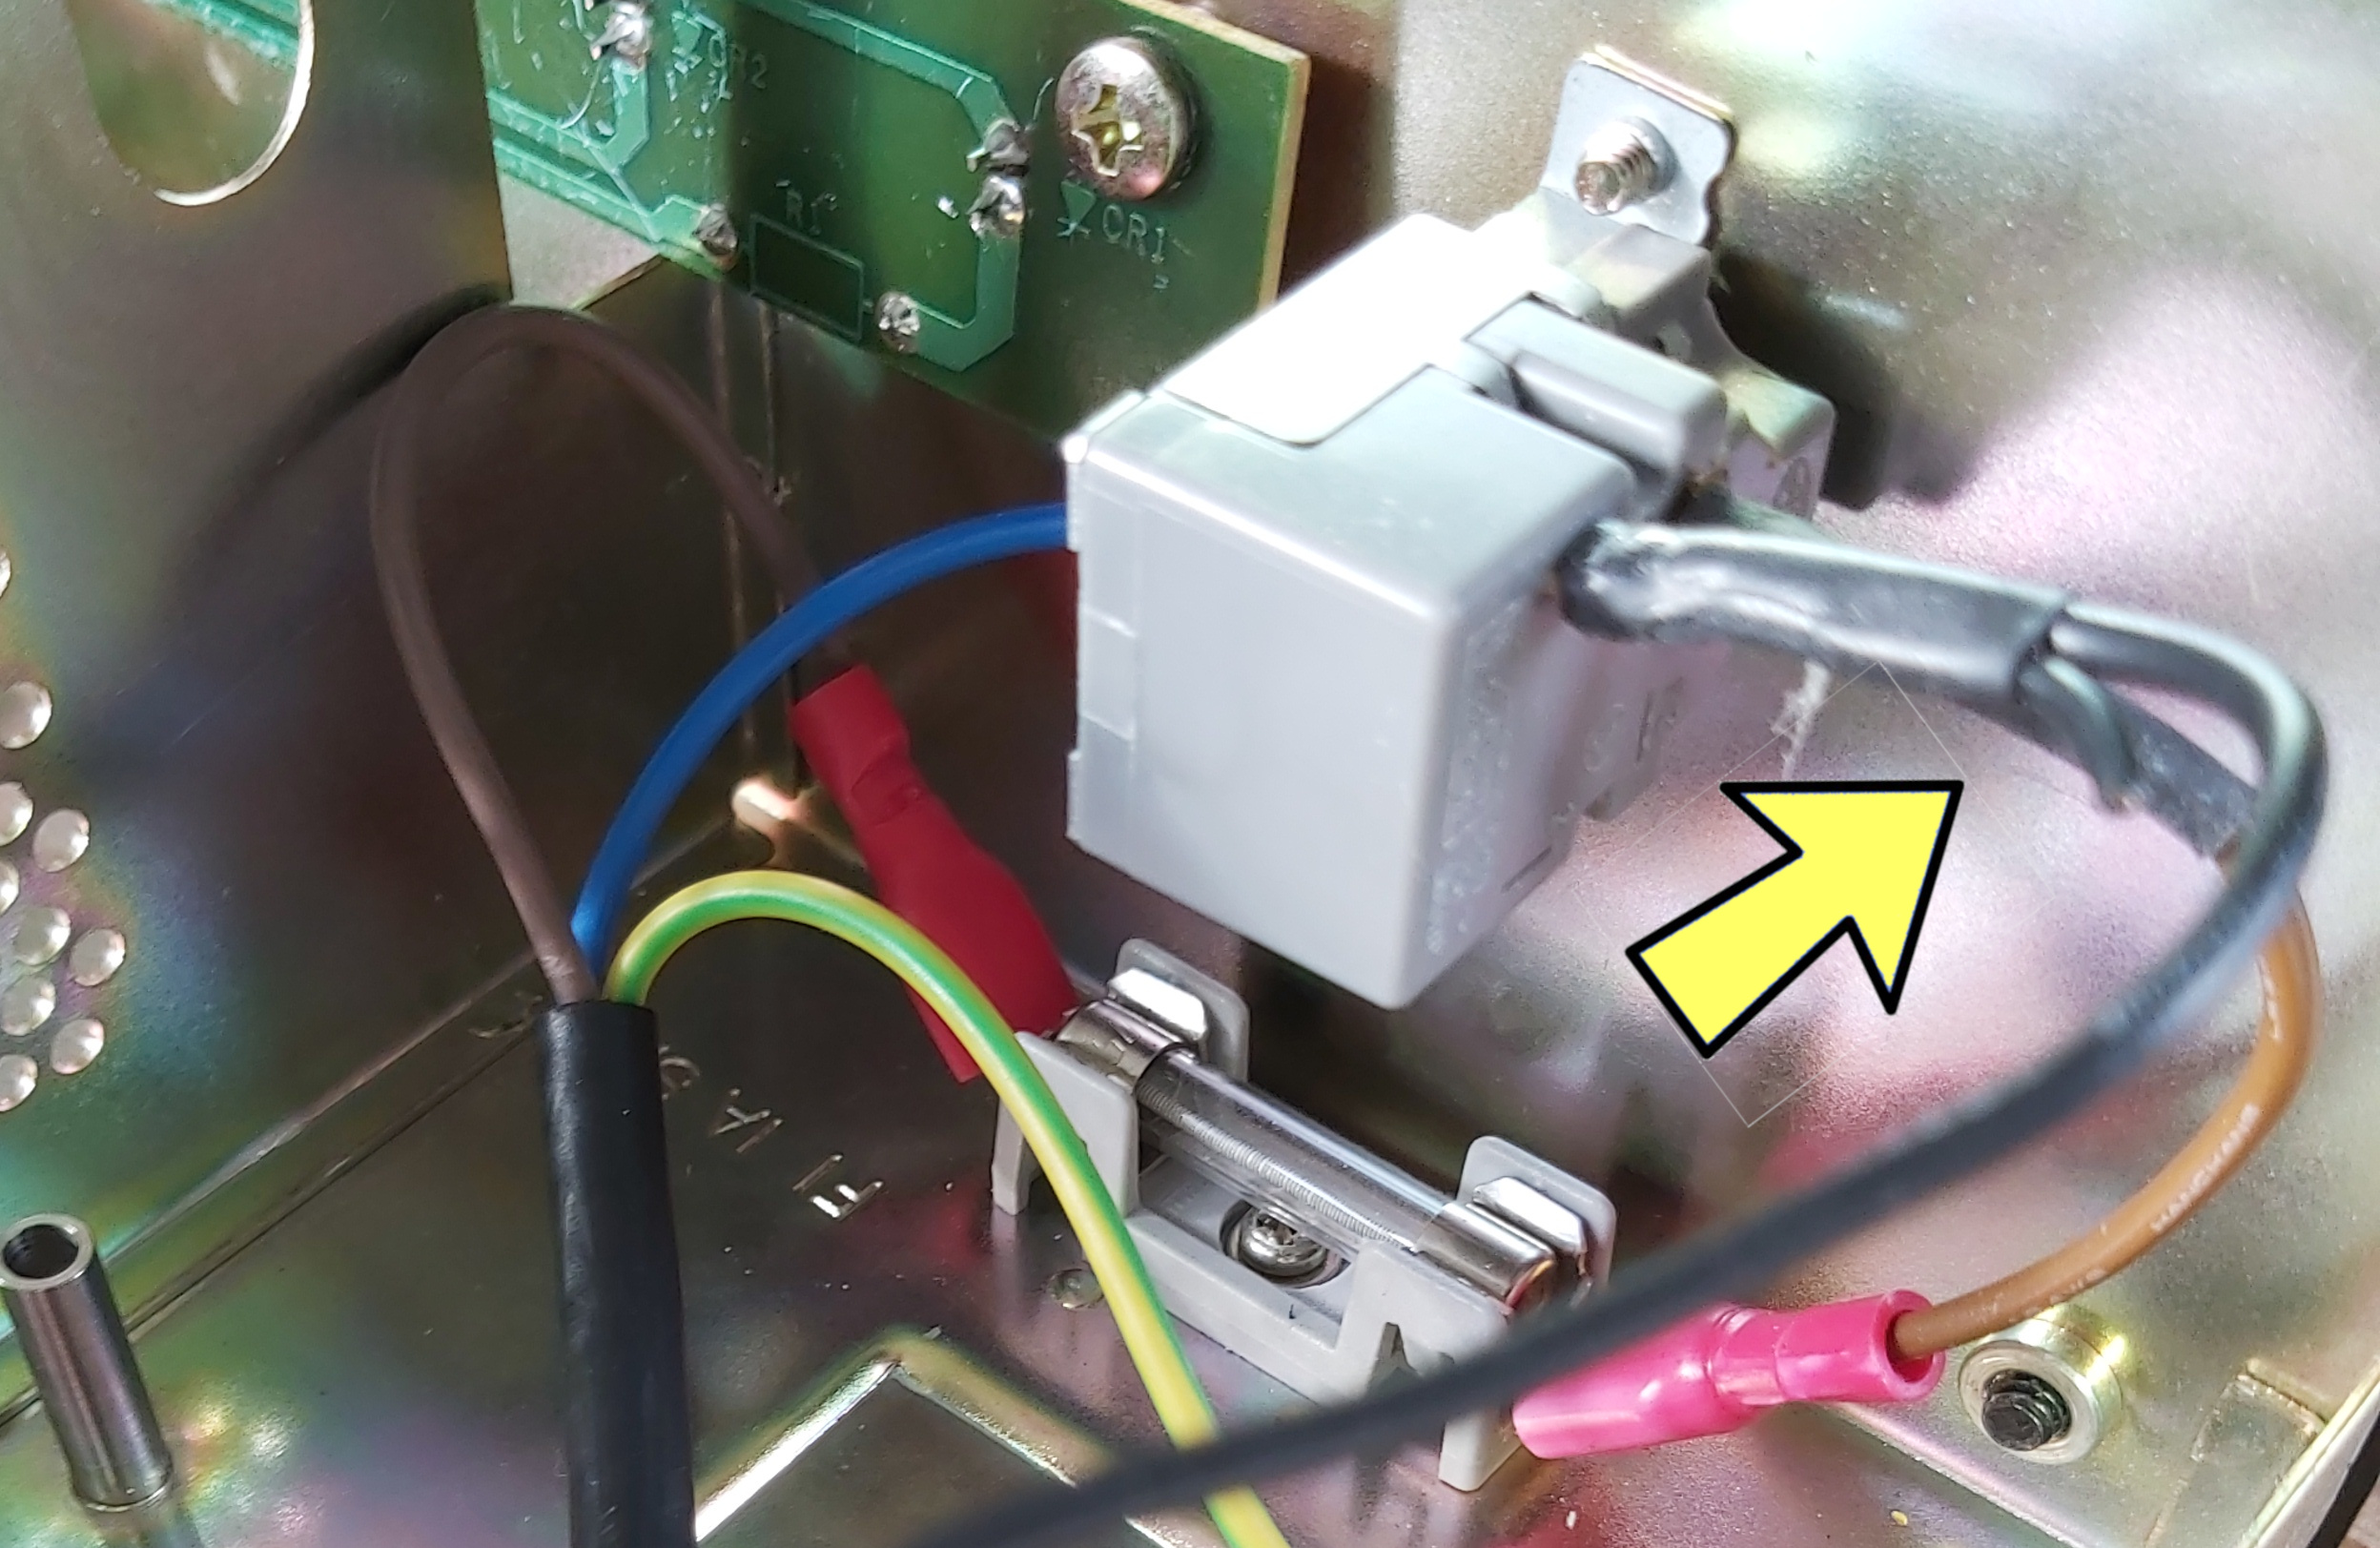
\includegraphics[width=\columnwidth]{images/psu-image-1a.jpg}
			\caption{Remove the remaining length of the fan power lead.}
			\label{fig:fan}
		\end{subfigure}
		\vskip1em
		\begin{subfigure}[b]{\columnwidth}
			%\end{figure}
			%\begin{figure}[t!]
			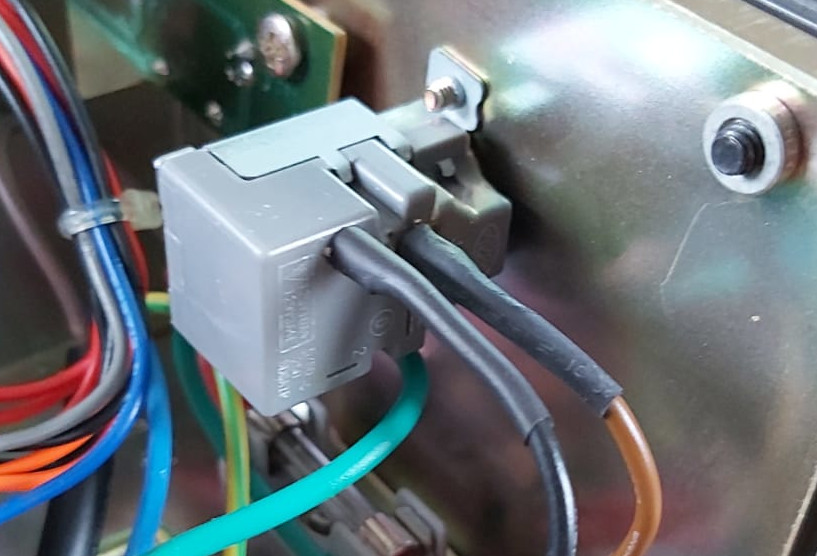
\includegraphics[width=\columnwidth]{images/psu-image-1b.jpg}
			\caption{Cover the power terminal with new heat shrink tubing.}
			\label{fig:tubing}
		\end{subfigure}
		\caption[Power button connection.]{Removing fan power lead.}
	\end{figure}
\end{enumerate}
\section{Replacing the mains cable}
The mains cable fitted to the NABU may be left in place and the Canada/US power plug replaced with a 3-pin domestic plug as appropriate. If the NABU cable is left in place, make note of the following colours and wire your domestic plug as shown in Table \ref{tbl:mains}.
\begin{center}
	\sffamily
	\begin{tblr}{
			colspec={|c|l|},
			hline{1,2,5},
			row{1} = {bg=gray4,fg=white,font=\bfseries},
			row{3} = {bg=gray9},
		}
		NABU lead & Function \\
		Green & Earth \\
		White & Neutral \\
		Black & Live \\
	\end{tblr}
	\taskLbl{tbl:mains}
	\taskTable{NABU mains lead details.}
\end{center}
Alternatively, the NABU mains cable can be replaced as following:
\begin{enumerate}
	\item Cut the NABU mains lead on the \textbf{inside} of the NABU system as close as possible to the strain relief bush grommet. Then pull the lead from the outside to free it from the grommet --- this may require some force and wriggling.
	\item Pass the new cable through the hole in the back of the case and secure it in place with the strain relief grommet recovered from the previous step. Allow enough length for the wires to comfortably reach the front of the NABU.
	\item Use a crimp tool to attach a ring connector to the mains Ground lead (green). Then attach a female spade connector to the Live lead (brown). Ensure that each connectors is securely attached to its lead to prevent poor contact.
	\item Firmly push the spade connector onto the fuse holder terminal. Loop the ring connector over the vertical `ground' post and secure it in place with a nut (as shown in Figure \ref{fig:new}). Note that the fuse itself does \textit{not} need to be replaced.
	\begin{figure}[h!]
		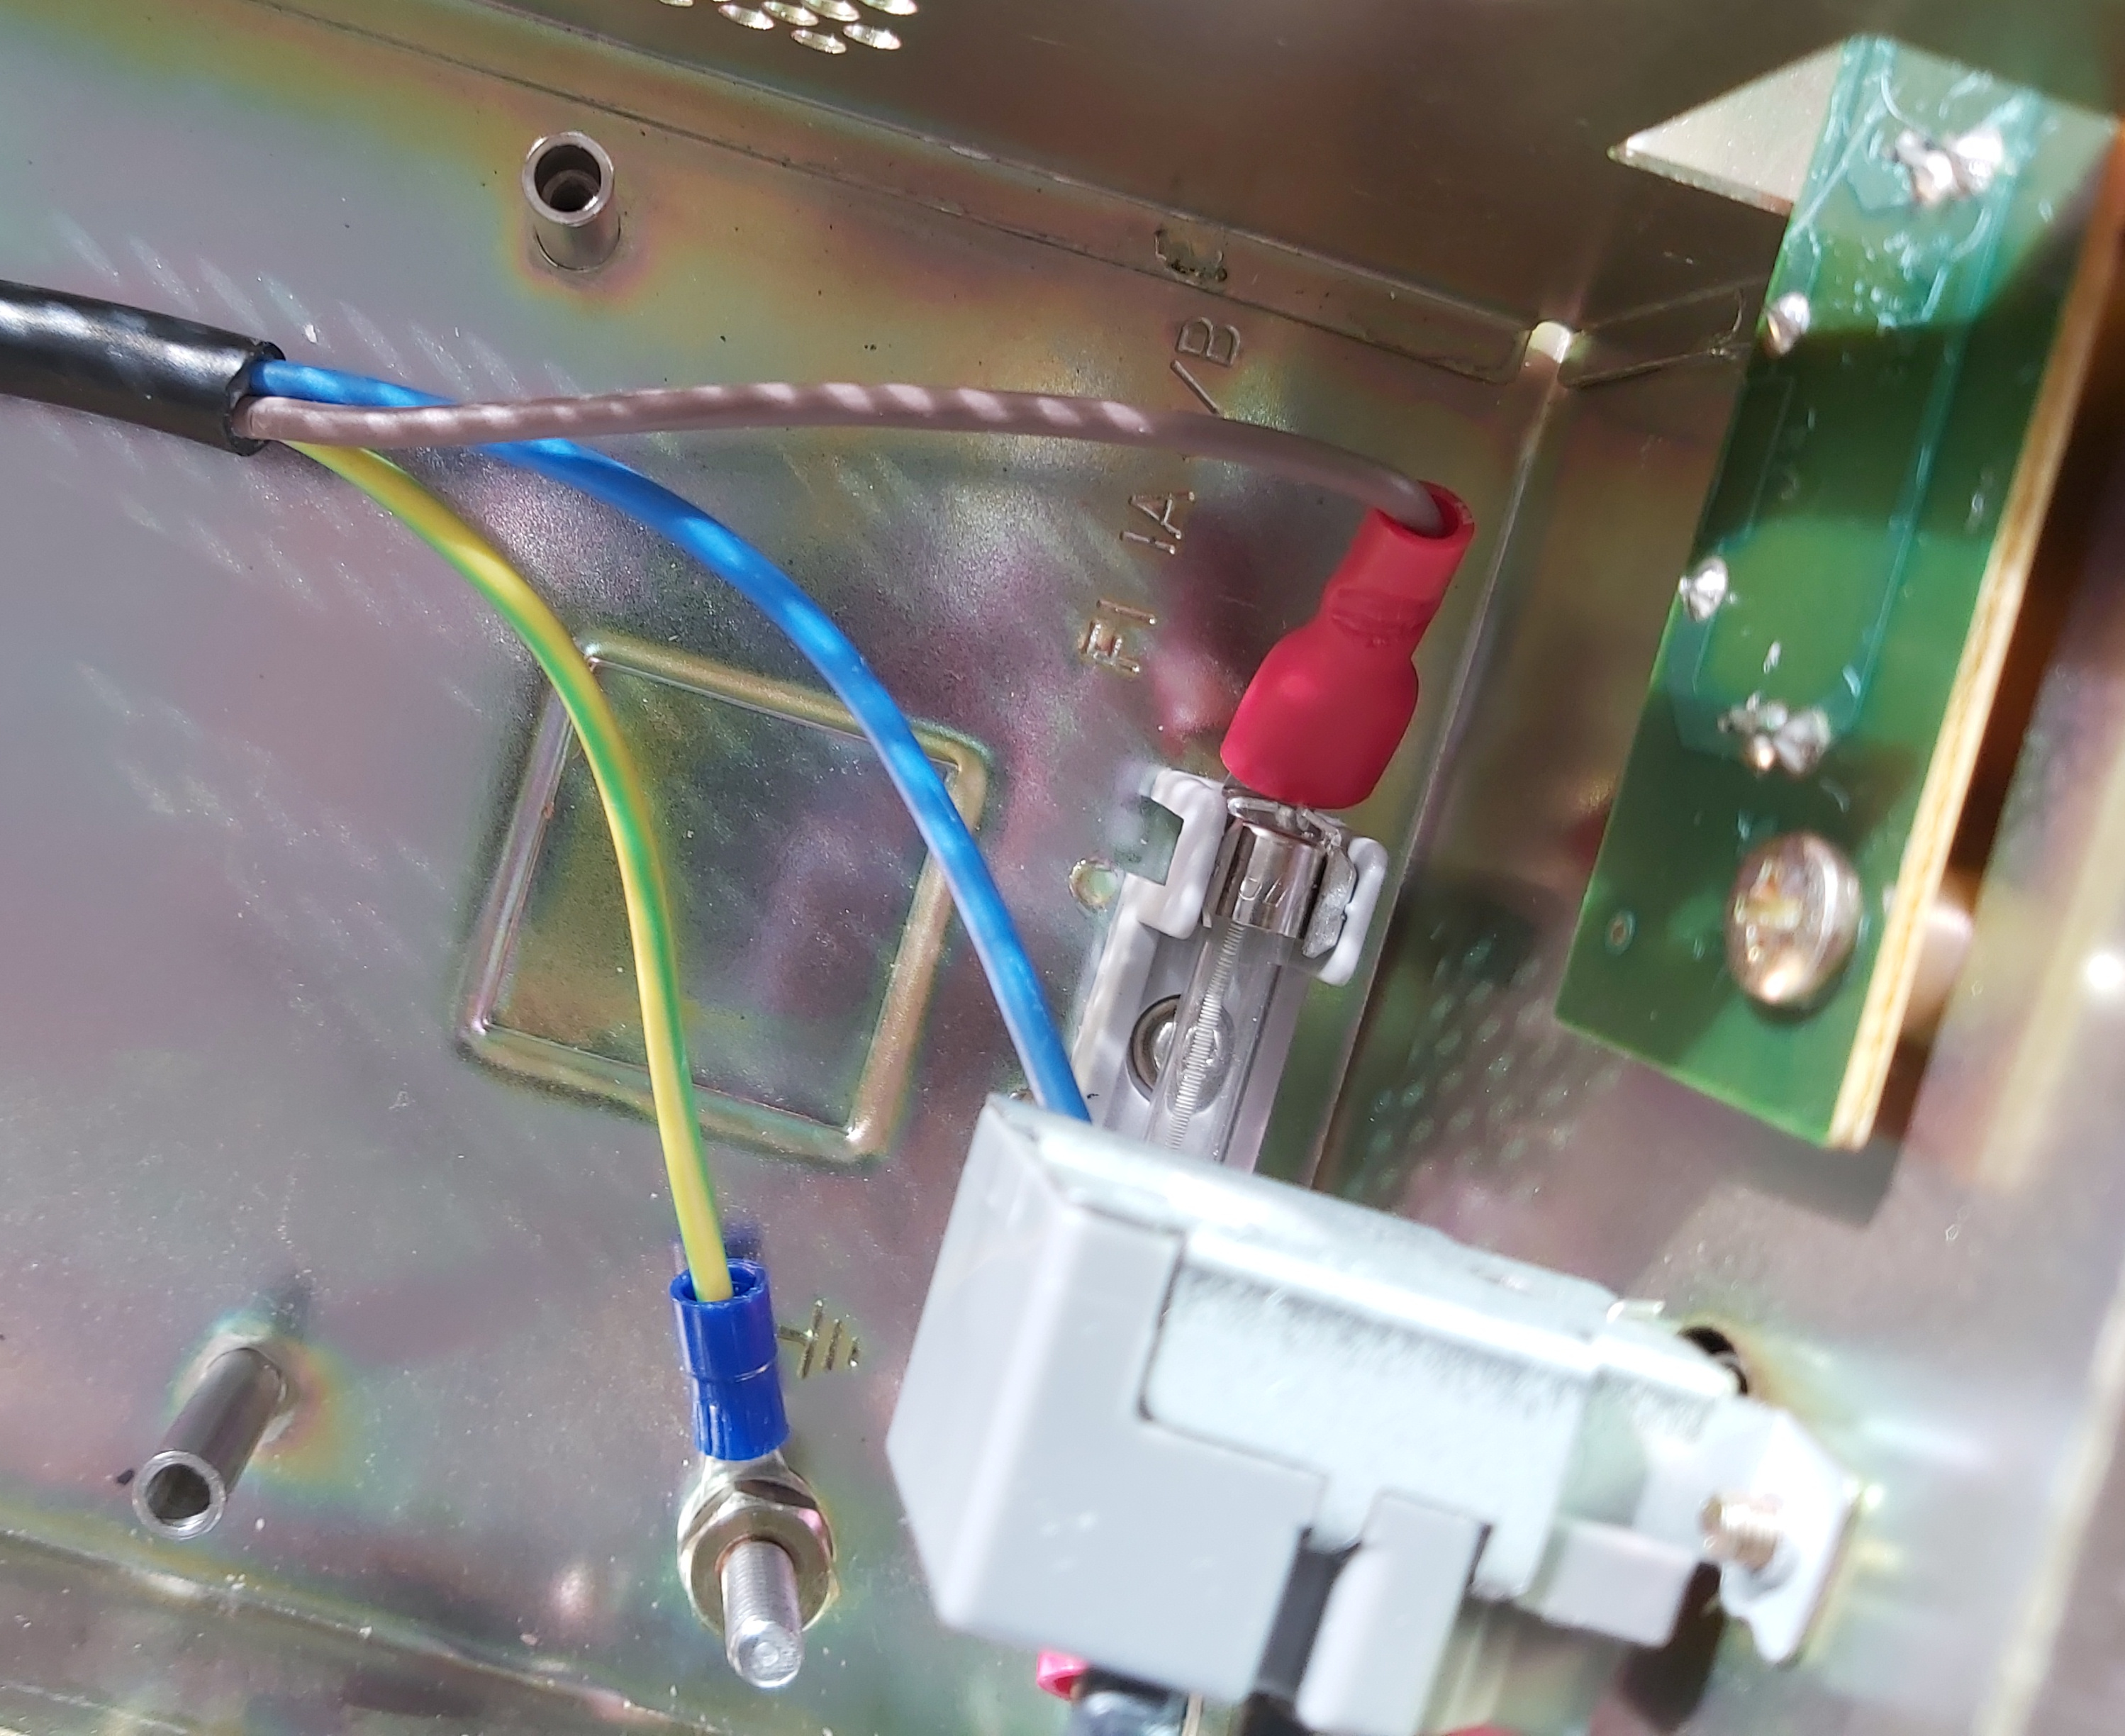
\includegraphics[width=\columnwidth]{images/psu-image-2.jpg}
		\caption[Ground and Live wire connections.]{Connect the Ground (green) and Live (brown) wires.}
		\label{fig:new}
	\end{figure}
\end{enumerate}
\section{Installing the Mean Well PSU}
The NABU requires multiple voltage levels, as detailed in the following table. The first two columns show the Mean Well RT-65B PSU terminals and their corresponding levels. The remaining columns show the colour and number of NABU wires that must be connected to each terminal. For example, both the single grey wire and two orange wires need to be connected to the terminal labelled \bbox{+V2} on the PSU.
\begin{center}
	\sffamily
	\begin{tblr}{
			colspec={|c|c|c|c|},
			hline{1,2,7},
			row{1} = {bg=gray4,fg=white,font=\bfseries},
			row{3,4,6} = {bg=gray9},
			cell{3}{1} = {r=2}{c},
			cell{3}{2} = {r=2}{c}
		}
		RT-65B & Level & Colour & Wires \\
		\bbox{V3} & -12V & Blue & 1 \\
		\bbox{+V2} & +12V & Grey & 1 \\
		& & Orange & 2 \\
		\bbox{COM} & Ground & Black & 3 \\
		\bbox{+5V} & +5V & Red & 3 \\
	\end{tblr}
	\taskLbl{tbl:wiring}
	\taskTable{Motherboard wiring details.}
\end{center}
To install the replacement PSU:
\begin{enumerate}
	\item If the mains cable was replaced, reattach the short ground lead (green) to the ground post and fix it in place with a nut.
	\item Place the Mean Well PSU such that the mounting hole near the \bbox{+5V Adj} trimmer on the PSU is lined up with the front right-hand post in the NABU bay and fix it in place with a screw. Note that the other posts do not line up with the remaining PSU mounting holes, meaning the PSU is kept in place with only a single screw.
	\item Attach the mains wires as shown. Be careful not to mix up the mains wires with the wires connected to the NABU motherboard.
	\begin{center}
		\sffamily
		\begin{tblr}{
				colspec={|c|c|c|},
				hline{1,2,5},
				row{1} = {bg=gray4,fg=white,font=\bfseries},
				row{3} = {bg=gray9}
			}
			RT-65B & Level & Colour \\
			\bbox{~L~\null} & Live & Black \\
			\bbox{~N~\null} & Neutral & Blue \\
			\bbox{~$\Ground$~\null} & Ground & Green \\
		\end{tblr}
		\taskLbl{tbl:live}
		\taskTable{Mains wiring details.}
	\end{center}
	\item Connect the wires leading from the NABU motherboard, as shown in Table \ref{tbl:wiring} (above) and Figure \ref{fig:terminals}.
	\begin{figure}[h!]
		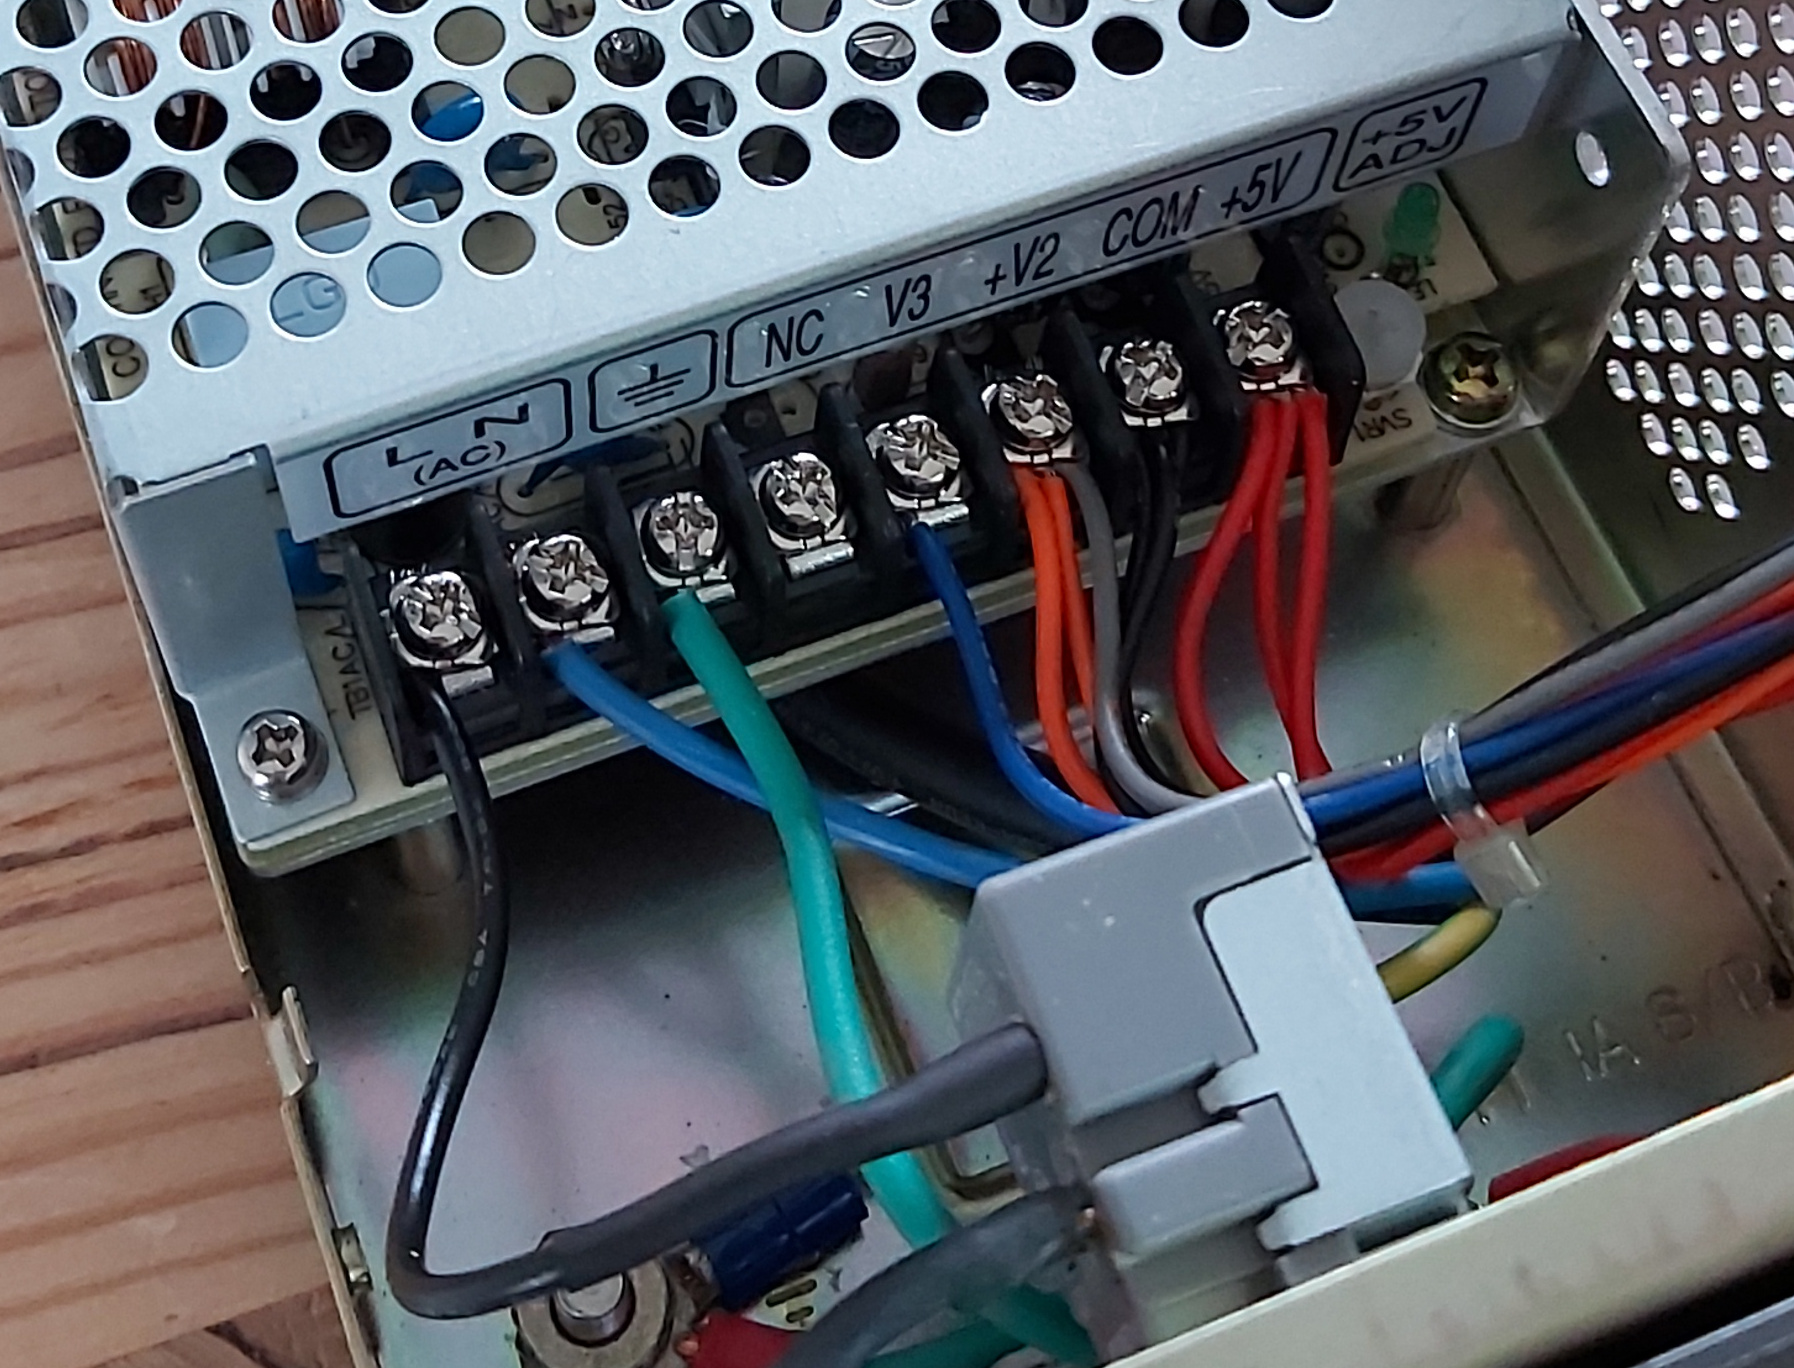
\includegraphics[width=\columnwidth]{images/psu-image-3.jpg}
		\caption[Motherboard to PSU wiring.]{Connect all wires to the relevant PSU terminals.}
		\label{fig:terminals}
	\end{figure}
	\item Connect the new fan leads to the PSU \bbox{COM} and either \bbox{+5V} or \bbox{+V2} terminals as appropriate.
	\item Check there are no loose parts or unconnected wires --- any wires that remain unconnected \textbf{and are no longer required} must be trimmed and made safe, e.g. by covering them with electrical insulation tape or heat shrink tubing. Once you are satisfied that all wires are correctly and securely connected, replace the NABU PSU cover and fix in place with its 2 screws.
	\item Replace the NABU system cover, securing it with 4 screws.
\end{enumerate}

\cleardoublepage

\end{document}